%% bare_conf.tex
%% V1.4b
%% 2015/08/26
%% by Michael Shell
%% See:
%% http://www.michaelshell.org/
%% for current contact information.
%%
%% This is a skeleton file demonstrating the use of IEEEtran.cls
%% (requires IEEEtran.cls version 1.8b or later) with an IEEE
%% conference paper.
%%
%% Support sites:
%% http://www.michaelshell.org/tex/ieeetran/
%% http://www.ctan.org/pkg/ieeetran
%% and
%% http://www.ieee.org/

%%*************************************************************************
%% Legal Notice:
%% This code is offered as-is without any warranty either expressed or
%% implied; without even the implied warranty of MERCHANTABILITY or
%% FITNESS FOR A PARTICULAR PURPOSE!
%% User assumes all risk.
%% In no event shall the IEEE or any contributor to this code be liable for
%% any damages or losses, including, but not limited to, incidental,
%% consequential, or any other damages, resulting from the use or misuse
%% of any information contained here.
%%
%% All comments are the opinions of their respective authors and are not
%% necessarily endorsed by the IEEE.
%%
%% This work is distributed under the LaTeX Project Public License (LPPL)
%% ( http://www.latex-project.org/ ) version 1.3, and may be freely used,
%% distributed and modified. A copy of the LPPL, version 1.3, is included
%% in the base LaTeX documentation of all distributions of LaTeX released
%% 2003/12/01 or later.
%% Retain all contribution notices and credits.
%% ** Modified files should be clearly indicated as such, including  **
%% ** renaming them and changing author support contact information. **
%%*************************************************************************


% *** Authors should verify (and, if needed, correct) their LaTeX system  ***
% *** with the testflow diagnostic prior to trusting their LaTeX platform ***
% *** with production work. The IEEE's font choices and paper sizes can   ***
% *** trigger bugs that do not appear when using other class files.       ***                          ***
% The testflow support page is at:
% http://www.michaelshell.org/tex/testflow/



\documentclass[conference]{IEEEtran}
% Some Computer Society conferences also require the compsoc mode option,
% but others use the standard conference format.
%
% If IEEEtran.cls has not been installed into the LaTeX system files,
% manually specify the path to it like:
% \documentclass[conference]{../sty/IEEEtran}





% Some very useful LaTeX packages include:
% (uncomment the ones you want to load)


% *** MISC UTILITY PACKAGES ***
%
%\usepackage{ifpdf}
% Heiko Oberdiek's ifpdf.sty is very useful if you need conditional
% compilation based on whether the output is pdf or dvi.
% usage:
% \ifpdf
%   % pdf code
% \else
%   % dvi code
% \fi
% The latest version of ifpdf.sty can be obtained from:
% http://www.ctan.org/pkg/ifpdf
% Also, note that IEEEtran.cls V1.7 and later provides a builtin
% \ifCLASSINFOpdf conditional that works the same way.
% When switching from latex to pdflatex and vice-versa, the compiler may
% have to be run twice to clear warning/error messages.






% *** CITATION PACKAGES ***
%
%\usepackage{cite}
% cite.sty was written by Donald Arseneau
% V1.6 and later of IEEEtran pre-defines the format of the cite.sty package
% \cite{} output to follow that of the IEEE. Loading the cite package will
% result in citation numbers being automatically sorted and properly
% "compressed/ranged". e.g., [1], [9], [2], [7], [5], [6] without using
% cite.sty will become [1], [2], [5]--[7], [9] using cite.sty. cite.sty's
% \cite will automatically add leading space, if needed. Use cite.sty's
% noadjust option (cite.sty V3.8 and later) if you want to turn this off
% such as if a citation ever needs to be enclosed in parenthesis.
% cite.sty is already installed on most LaTeX systems. Be sure and use
% version 5.0 (2009-03-20) and later if using hyperref.sty.
% The latest version can be obtained at:
% http://www.ctan.org/pkg/cite
% The documentation is contained in the cite.sty file itself.






% *** GRAPHICS RELATED PACKAGES ***
%
\ifCLASSINFOpdf
  % \usepackage[pdftex]{graphicx}
  % declare the path(s) where your graphic files are
  % \graphicspath{{../pdf/}{../jpeg/}}
  % and their extensions so you won't have to specify these with
  % every instance of \includegraphics
  % \DeclareGraphicsExtensions{.pdf,.jpeg,.png}
\else
  % or other class option (dvipsone, dvipdf, if not using dvips). graphicx
  % will default to the driver specified in the system graphics.cfg if no
  % driver is specified.
  % \usepackage[dvips]{graphicx}
  % declare the path(s) where your graphic files are
  % \graphicspath{{../eps/}}
  % and their extensions so you won't have to specify these with
  % every instance of \includegraphics
  % \DeclareGraphicsExtensions{.eps}
\fi
% graphicx was written by David Carlisle and Sebastian Rahtz. It is
% required if you want graphics, photos, etc. graphicx.sty is already
% installed on most LaTeX systems. The latest version and documentation
% can be obtained at:
% http://www.ctan.org/pkg/graphicx
% Another good source of documentation is "Using Imported Graphics in
% LaTeX2e" by Keith Reckdahl which can be found at:
% http://www.ctan.org/pkg/epslatex
%
% latex, and pdflatex in dvi mode, support graphics in encapsulated
% postscript (.eps) format. pdflatex in pdf mode supports graphics
% in .pdf, .jpeg, .png and .mps (metapost) formats. Users should ensure
% that all non-photo figures use a vector format (.eps, .pdf, .mps) and
% not a bitmapped formats (.jpeg, .png). The IEEE frowns on bitmapped formats
% which can result in "jaggedy"/blurry rendering of lines and letters as
% well as large increases in file sizes.
%
% You can find documentation about the pdfTeX application at:
% http://www.tug.org/applications/pdftex





% *** MATH PACKAGES ***
%
%\usepackage{amsmath}
% A popular package from the American Mathematical Society that provides
% many useful and powerful commands for dealing with mathematics.
%
% Note that the amsmath package sets \interdisplaylinepenalty to 10000
% thus preventing page breaks from occurring within multiline equations. Use:
%\interdisplaylinepenalty=2500
% after loading amsmath to restore such page breaks as IEEEtran.cls normally
% does. amsmath.sty is already installed on most LaTeX systems. The latest
% version and documentation can be obtained at:
% http://www.ctan.org/pkg/amsmath





% *** SPECIALIZED LIST PACKAGES ***
%
%\usepackage{algorithmic}
% algorithmic.sty was written by Peter Williams and Rogerio Brito.
% This package provides an algorithmic environment fo describing algorithms.
% You can use the algorithmic environment in-text or within a figure
% environment to provide for a floating algorithm. Do NOT use the algorithm
% floating environment provided by algorithm.sty (by the same authors) or
% algorithm2e.sty (by Christophe Fiorio) as the IEEE does not use dedicated
% algorithm float types and packages that provide these will not provide
% correct IEEE style captions. The latest version and documentation of
% algorithmic.sty can be obtained at:
% http://www.ctan.org/pkg/algorithms
% Also of interest may be the (relatively newer and more customizable)
% algorithmicx.sty package by Szasz Janos:
% http://www.ctan.org/pkg/algorithmicx




% *** ALIGNMENT PACKAGES ***
%
%\usepackage{array}
% Frank Mittelbach's and David Carlisle's array.sty patches and improves
% the standard LaTeX2e array and tabular environments to provide better
% appearance and additional user controls. As the default LaTeX2e table
% generation code is lacking to the point of almost being broken with
% respect to the quality of the end results, all users are strongly
% advised to use an enhanced (at the very least that provided by array.sty)
% set of table tools. array.sty is already installed on most systems. The
% latest version and documentation can be obtained at:
% http://www.ctan.org/pkg/array


% IEEEtran contains the IEEEeqnarray family of commands that can be used to
% generate multiline equations as well as matrices, tables, etc., of high
% quality.




% *** SUBFIGURE PACKAGES ***
%\ifCLASSOPTIONcompsoc
%  \usepackage[caption=false,font=normalsize,labelfont=sf,textfont=sf]{subfig}
%\else
%  \usepackage[caption=false,font=footnotesize]{subfig}
%\fi
% subfig.sty, written by Steven Douglas Cochran, is the modern replacement
% for subfigure.sty, the latter of which is no longer maintained and is
% incompatible with some LaTeX packages including fixltx2e. However,
% subfig.sty requires and automatically loads Axel Sommerfeldt's caption.sty
% which will override IEEEtran.cls' handling of captions and this will result
% in non-IEEE style figure/table captions. To prevent this problem, be sure
% and invoke subfig.sty's "caption=false" package option (available since
% subfig.sty version 1.3, 2005/06/28) as this is will preserve IEEEtran.cls
% handling of captions.
% Note that the Computer Society format requires a larger sans serif font
% than the serif footnote size font used in traditional IEEE formatting
% and thus the need to invoke different subfig.sty package options depending
% on whether compsoc mode has been enabled.
%
% The latest version and documentation of subfig.sty can be obtained at:
% http://www.ctan.org/pkg/subfig




% *** FLOAT PACKAGES ***
%
%\usepackage{fixltx2e}
% fixltx2e, the successor to the earlier fix2col.sty, was written by
% Frank Mittelbach and David Carlisle. This package corrects a few problems
% in the LaTeX2e kernel, the most notable of which is that in current
% LaTeX2e releases, the ordering of single and double column floats is not
% guaranteed to be preserved. Thus, an unpatched LaTeX2e can allow a
% single column figure to be placed prior to an earlier double column
% figure.
% Be aware that LaTeX2e kernels dated 2015 and later have fixltx2e.sty's
% corrections already built into the system in which case a warning will
% be issued if an attempt is made to load fixltx2e.sty as it is no longer
% needed.
% The latest version and documentation can be found at:
% http://www.ctan.org/pkg/fixltx2e


%\usepackage{stfloats}
% stfloats.sty was written by Sigitas Tolusis. This package gives LaTeX2e
% the ability to do double column floats at the bottom of the page as well
% as the top. (e.g., "\begin{figure*}[!b]" is not normally possible in
% LaTeX2e). It also provides a command:
%\fnbelowfloat
% to enable the placement of footnotes below bottom floats (the standard
% LaTeX2e kernel puts them above bottom floats). This is an invasive package
% which rewrites many portions of the LaTeX2e float routines. It may not work
% with other packages that modify the LaTeX2e float routines. The latest
% version and documentation can be obtained at:
% http://www.ctan.org/pkg/stfloats
% Do not use the stfloats baselinefloat ability as the IEEE does not allow
% \baselineskip to stretch. Authors submitting work to the IEEE should note
% that the IEEE rarely uses double column equations and that authors should try
% to avoid such use. Do not be tempted to use the cuted.sty or midfloat.sty
% packages (also by Sigitas Tolusis) as the IEEE does not format its papers in
% such ways.
% Do not attempt to use stfloats with fixltx2e as they are incompatible.
% Instead, use Morten Hogholm'a dblfloatfix which combines the features
% of both fixltx2e and stfloats:
%
% \usepackage{dblfloatfix}
% The latest version can be found at:
% http://www.ctan.org/pkg/dblfloatfix




% *** PDF, URL AND HYPERLINK PACKAGES ***
%
%\usepackage{url}
% url.sty was written by Donald Arseneau. It provides better support for
% handling and breaking URLs. url.sty is already installed on most LaTeX
% systems. The latest version and documentation can be obtained at:
% http://www.ctan.org/pkg/url
% Basically, \url{my_url_here}.




% *** Do not adjust lengths that control margins, column widths, etc. ***
% *** Do not use packages that alter fonts (such as pslatex).         ***
% There should be no need to do such things with IEEEtran.cls V1.6 and later.
% (Unless specifically asked to do so by the journal or conference you plan
% to submit to, of course. )


% correct bad hyphenation here
\hyphenation{op-tical net-works semi-conduc-tor}

\usepackage{fancyhdr}
\usepackage{hyperref}
\usepackage{bbm}
\usepackage{times}
\usepackage{xcolor}
\usepackage{soul}
\usepackage[utf8]{inputenc}
%\usepackage[small]{caption}
\usepackage{latexsym} 
\usepackage{amsmath}
\usepackage{graphicx}
%\usepackage[style=base]{caption}
%\usepackage{caption}
\usepackage{subcaption}
\usepackage{array}
\usepackage{amsmath}
\usepackage{amsfonts}
\usepackage{graphicx}
\usepackage[colorinlistoftodos]{todonotes}
\usepackage{algorithm}
\usepackage{algpseudocode}
\graphicspath{ {images/} }
\usepackage[square,sort,comma,numbers]{natbib}
\usepackage{geometry}
 \geometry{
 a4paper,
 %total={210mm,297mm},
 left=20mm,
 right=20mm,
 top=20mm,
 bottom=20mm,
 }
\usepackage{setspace}

\usepackage{graphicx,epstopdf}
\epstopdfsetup{update}
\DeclareGraphicsExtensions{.ps}
\epstopdfDeclareGraphicsRule{.ps}{pdf}{.pdf}{ps2pdf -dEPSCrop -dNOSAFER #1 \OutputFile}


% Ensure letter paper
\pdfpagewidth=8.5in
\pdfpageheight=11in

% commands
\newcommand{\ignore}[1]{}

%%%%%%%%%%%---SETME-----%%%%%%%%%%%%%
\newcommand{\microsubmissionnumber}{XXX}
%%%%%%%%%%%%%%%%%%%%%%%%%%%%%%%%%%%%
\fancypagestyle{firstpage}{
  \fancyhf{}
\setlength{\headheight}{12pt}
\renewcommand{\headrulewidth}{0pt}
  \fancyhead[C]{\normalsize{MICRO 2018 Submission
      \textbf{\#\microsubmissionnumber} -- Confidential Draft -- Do NOT Distribute!!}}
  \pagenumbering{arabic}
}

%%%%%%%%%%---SETME-----%%%%%%%%%%%%%
\title{SMART: Runtime Support for Personalized AI}
\author{\IEEEauthorblockN{Boyuan Feng}
\IEEEauthorblockA{boyuan@cs.ucsb.edu}
\and
\IEEEauthorblockN{Kun Wan}
\IEEEauthorblockA{kun@cs.ucsb.edu}
\and
\IEEEauthorblockN{Yufei Ding}
\IEEEauthorblockA{yufeiding@cs.ucsb.edu}
}
%\affil{Department of Computer Science \\
%University of California, Santa Barbara}


%%%%%%%%%%%%%%%%%%%%%%%%%%%%%%%%%%%%
\begin{document}
\begin{spacing}{0.9}
%
% paper title
% Titles are generally capitalized except for words such as a, an, and, as,
% at, but, by, for, in, nor, of, on, or, the, to and up, which are usually
% not capitalized unless they are the first or last word of the title.
% Linebreaks \\ can be used within to get better formatting as desired.
% Do not put math or special symbols in the title.



% author names and affiliations
% use a multiple column layout for up to three different
% affiliations
%\author{\IEEEauthorblockN{Michael Shell}
%\IEEEauthorblockA{School of Electrical and\\Computer Engineering\\
%Georgia Institute of Technology\\
%Atlanta, Georgia 30332--0250\\
%Email: http://www.michaelshell.org/contact.html}
%\and
%\IEEEauthorblockN{Homer Simpson}
%\IEEEauthorblockA{Twentieth Century Fox\\
%Springfield, USA\\
%Email: homer@thesimpsons.com}
%\and
%\IEEEauthorblockN{James Kirk\\ and Montgomery Scott}
%\IEEEauthorblockA{Starfleet Academy\\
%San Francisco, California 96678--2391\\
%Telephone: (800) 555--1212\\
%Fax: (888) 555--1212}}

% conference papers do not typically use \thanks and this command
% is locked out in conference mode. If really needed, such as for
% the acknowledgment of grants, issue a \IEEEoverridecommandlockouts
% after \documentclass

% for over three affiliations, or if they all won't fit within the width
% of the page, use this alternative format:
%
%\author{\IEEEauthorblockN{Michael Shell\IEEEauthorrefmark{1},
%Homer Simpson\IEEEauthorrefmark{2},
%James Kirk\IEEEauthorrefmark{3},
%Montgomery Scott\IEEEauthorrefmark{3} and
%Eldon Tyrell\IEEEauthorrefmark{4}}
%\IEEEauthorblockA{\IEEEauthorrefmark{1}School of Electrical and Computer Engineering\\
%Georgia Institute of Technology,
%Atlanta, Georgia 30332--0250\\ Email: see http://www.michaelshell.org/contact.html}
%\IEEEauthorblockA{\IEEEauthorrefmark{2}Twentieth Century Fox, Springfield, USA\\
%Email: homer@thesimpsons.com}
%\IEEEauthorblockA{\IEEEauthorrefmark{3}Starfleet Academy, San Francisco, California 96678-2391\\
%Telephone: (800) 555--1212, Fax: (888) 555--1212}
%\IEEEauthorblockA{\IEEEauthorrefmark{4}Tyrell Inc., 123 Replicant Street, Los Angeles, California 90210--4321}}




% use for special paper notices
%\IEEEspecialpapernotice{(Invited Paper)}




% make the title area
\maketitle
\thispagestyle{firstpage}
\pagestyle{plain}


%%%%%% -- PAPER CONTENT STARTS-- %%%%%%%%
% As a general rule, do not put math, special symbols or citations
% in the abstract
\begin{abstract}
    Runtime class distribution is an essential part in energy-efficient deployment of CNN models on mobile device. Unfortunately, existing papers only focus on the number of classes and overlook the importance of \textit{class correlation}. Unlike such qualitative description as reducing number of classes can increase accuracy, our principles are quantitative: a metric has been proposed to measure \textit{class correlation}. Based on the \textit{quantitative metric}, \textit{guided search} is brought up to replace the existing method \textit{exhaustive search} and thus reduce tons of overhead. Further, \textit{probability layer} is proposed to avoid runtime retraining. We formulate the problem of adjust models according to runtime distribution and energy budget into a scheduling problem and bring up a runtime supporting framework, called \textit{SMART}, to choose model automatically.
\end{abstract}

% no keywords


% For peer review papers, you can put extra information on the cover
% page as needed:
% \ifCLASSOPTIONpeerreview
% \begin{center} \bfseries EDICS Category: 3-BBND \end{center}
% \fi
%
% For peerreview papers, this IEEEtran command inserts a page break and
% creates the second title. It will be ignored for other modes.
%\IEEEpeerreviewmaketitle


\section{Introduction}
Image classification is an important area due to their abundant applications in daily life. In recent years, unprecedented advance has been made and the state-of-the-art CNN models can even beat human's accuracy \cite{russakovsky2015imagenet} on image classification. These CNN models are expected to be employed on mobile devices and give personalized suggestions. For example, AI-powered smart glasses are desired to detect different types of objects, identify current environment, and give user real-time suggestion. The obstacle to this exciting perspective is energy efficiency problem. The mobile device cannot serve CNN models due to the huge consumption of energy and memory. On solving this energy efficiency problem, runtime class skew has been found to be an effective method. \cite{han2016mcdnn} and \cite{shen2016fast} report that reducing number of classes can both increase accuracy and reduce resource consumption. Actually, only a small portion of classes can be seen in a specific scenario even if the CNNs tested in lab environment target thousands of classes. This method is called \textit{runtime class skew}, since class skew could only be observed when a specific is using the device and cannot be predicted in lab environment.

We extend previous papers from only considering number of classes to incorporating similarity between classes, called \textit{class correlation}. Figure \ref{fig:classEffect} shows the intuition that classifying house, cat, dog, and tree is much easier than distinguishing four different cat species. Through a series of experiments, we found that classes with low \textit{class correlation} have much higher testing accuracy than classes with high \textit{class correlation} even if the model architecture and the number of classes remain unchaned. While number of classes consider how many classes have appeared in a scenario, \textit{class correlation} considers how similar the group of classes are to each other, which is orthogonal to number of classes. To model the class correlation, a semantic tree representing closeness of labels in semantic is a straightforward idea. However, the way that algorithms found similarity is largely different from human's feeling. Thus a much more advanced quantitative method, \textit{QuantClosenesses}, has been proposed to mimic the thinking process of CNN models. 

\begin{figure} 
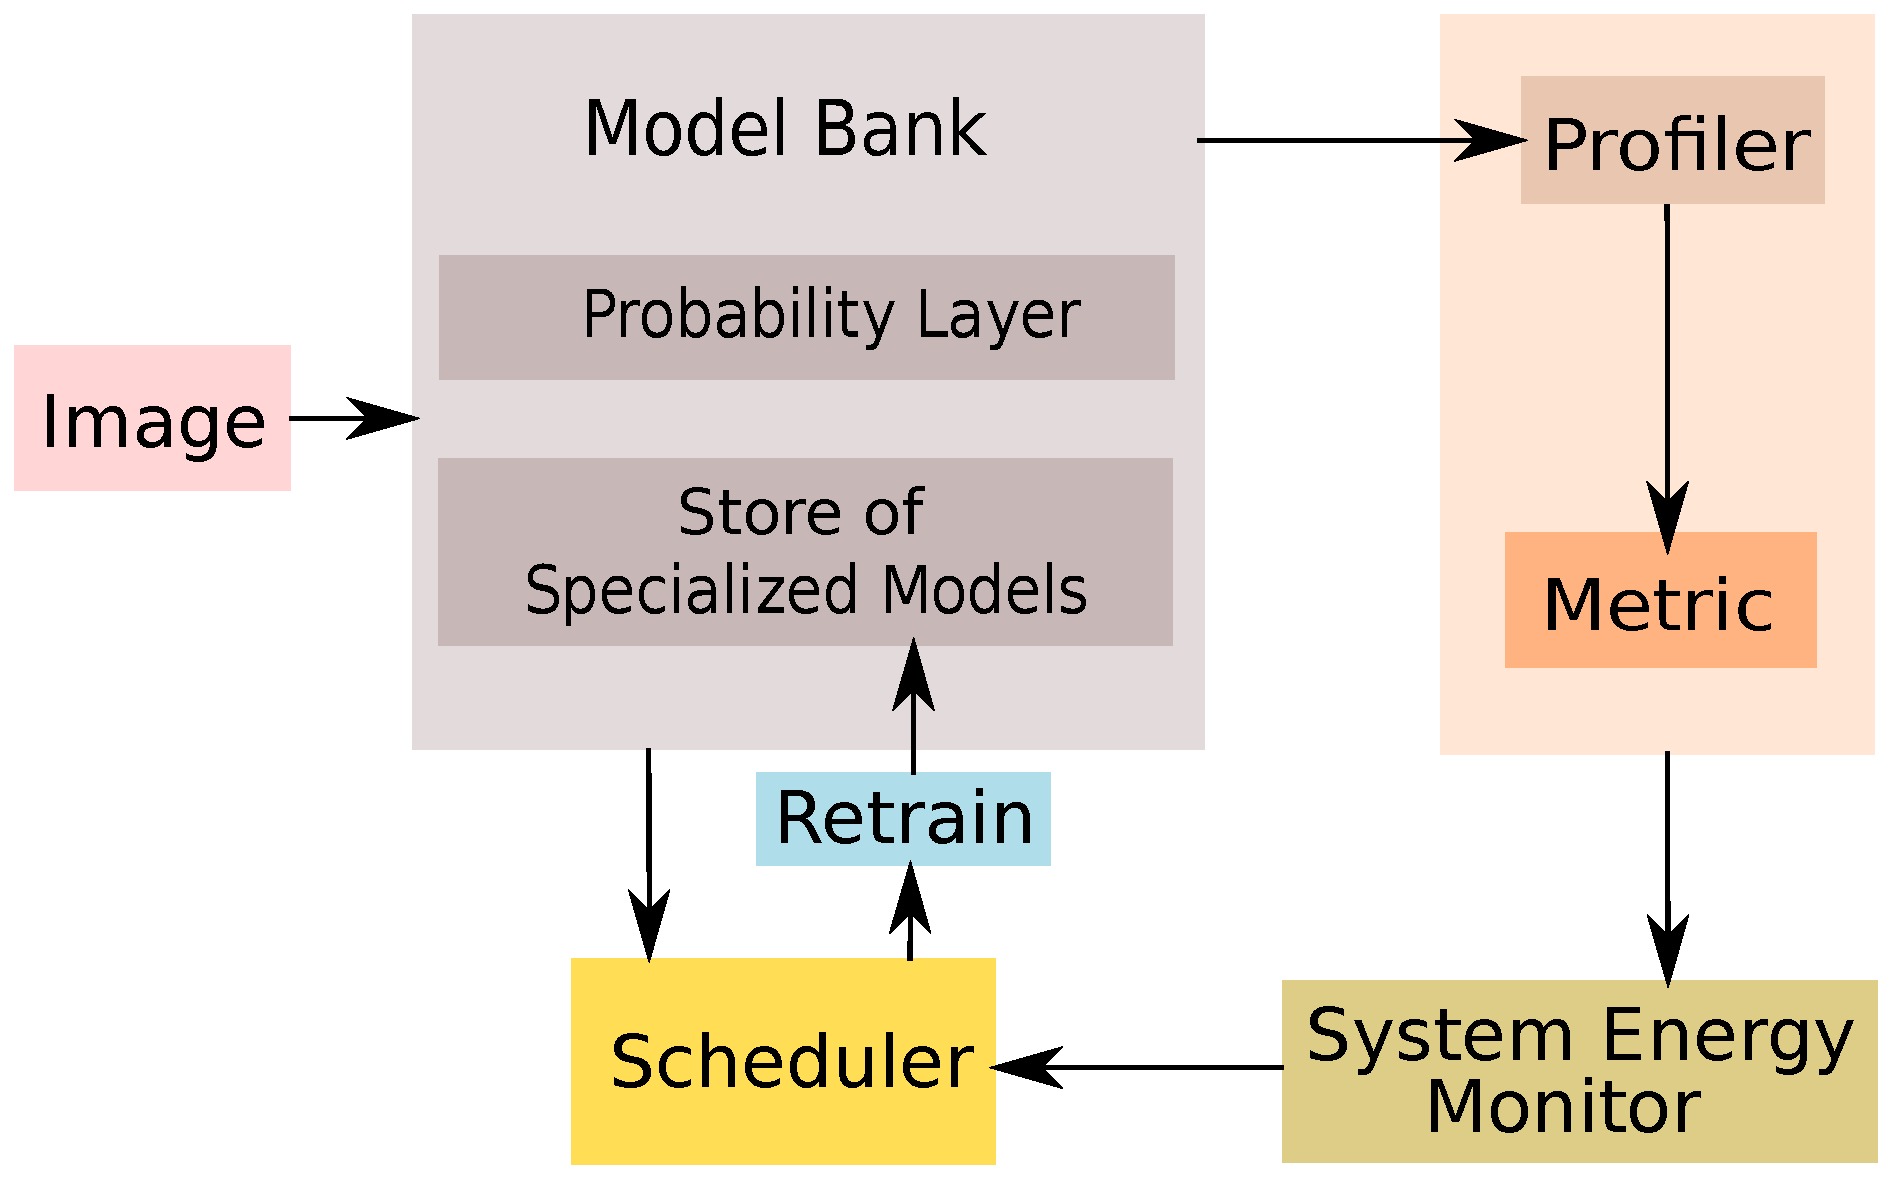
\includegraphics[scale=0.25]{complexArchitecture.ps}
\caption{Overall architecture: This graph shows the overall architecture of SMART framework. The input are images. Every image will be forwarded into the scheduler. The scheduler first refers to the profiler and check whether there is a class skew. Then the scheduler will estimate the energy constraint for this image and choose the model with best accuracy given this energy constraint. The executor will follow the scheduler's decision and grasp the corresponding model from model store, which is a on-disk storage of previous train-ed models. Finally, the predicted value will be recorded by profiler for future usage.}
\label{fig:Architecture}
\end{figure}


\begin{figure*}
\centering
\begin{subfigure}{.15\textwidth}
  \centering
  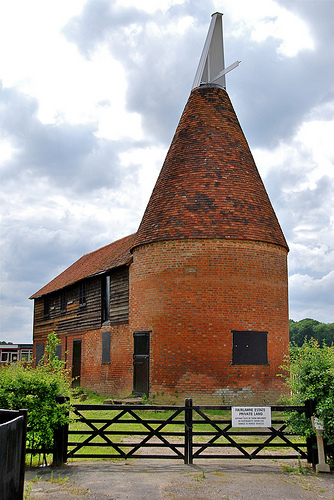
\includegraphics[scale=0.1]{classTypeExample1.jpg}
  \caption{House}
\end{subfigure}%
\begin{subfigure}{.15\textwidth}
  \centering
  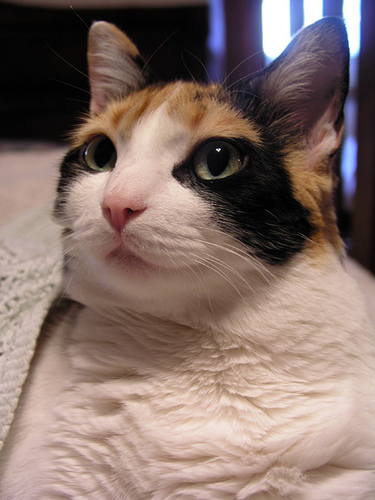
\includegraphics[scale=0.14]{classTypeExample2.jpg}
  \caption{Cat}
\end{subfigure}%
\begin{subfigure}{.15\textwidth}
  \centering
  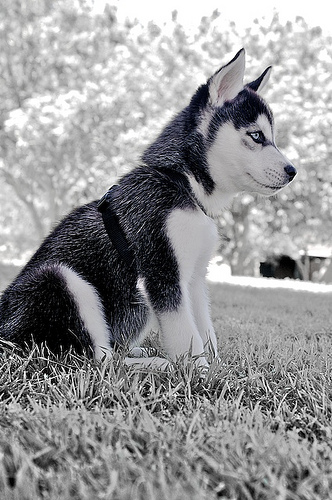
\includegraphics[scale=0.1]{classTypeExample3.jpg}
  \caption{Dog}
\end{subfigure}%
\begin{subfigure}{.15\textwidth}
  \centering
  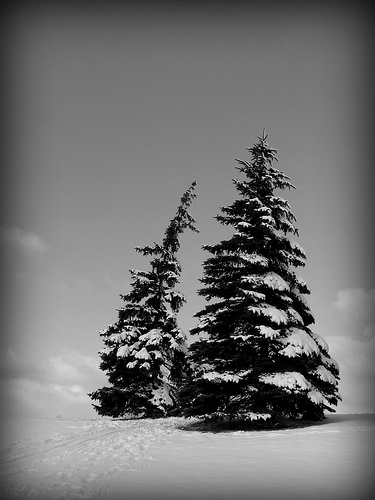
\includegraphics[scale=0.1]{classTypeExample4.jpg}
  \caption{Tree}
\end{subfigure}
\begin{subfigure}{.15\textwidth}
  \centering
  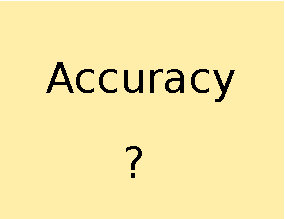
\includegraphics[scale=0.3]{Accuracy.ps}
\end{subfigure}


\begin{subfigure}{.15\textwidth}
  \centering
  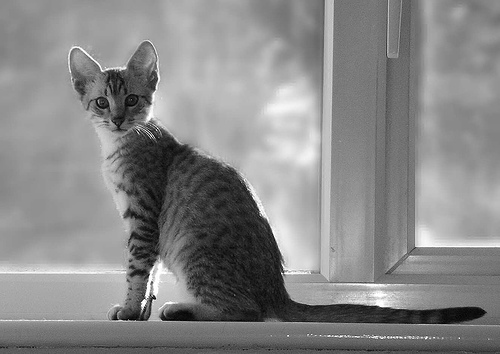
\includegraphics[scale=0.1]{classTypeExample5.jpg}
  \caption{Egyptian Cat}
\end{subfigure}
\begin{subfigure}{.15\textwidth}
  \centering
  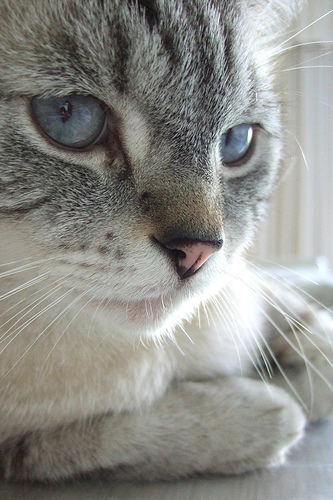
\includegraphics[scale=0.11]{classTypeExample6.jpg}
  \caption{Kitty Cat}
\end{subfigure}
\begin{subfigure}{.15\textwidth}
  \centering
  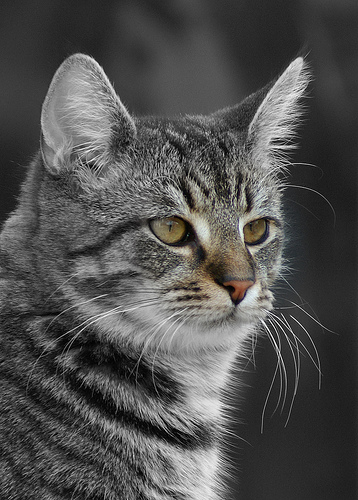
\includegraphics[scale=0.15]{classTypeExample7.jpg}
  \caption{Tiger Cat}
\end{subfigure}
\begin{subfigure}{.15\textwidth}
  \centering
  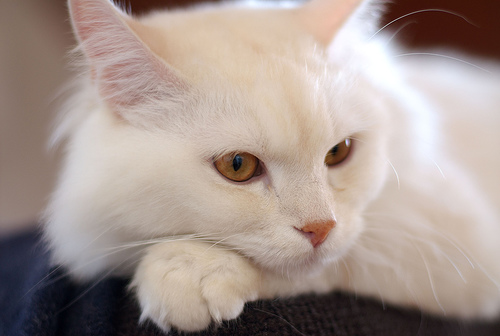
\includegraphics[scale=0.1]{classTypeExample8.jpg}
  \caption{Angora Cat}
\end{subfigure}
\begin{subfigure}{.15\textwidth}
  \centering
  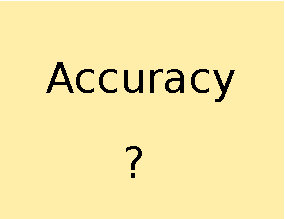
\includegraphics[scale=0.3]{Accuracy.ps}
\end{subfigure}

\caption{This set of images shows the class effect. It is much easier to distinguish house, cat, dog, and tree than classifying four cat species using the same architecture. This observation meets our intuition.}
\label{fig:classEffect}
\end{figure*}




The improvement on accuracy brought in by class skew provides the space for model simplification. There are two difference between our work and existing papers \cite{han2016mcdnn, kang2017noscope}. The first difference is how to search candidate models: we use guided search while existing papers use exhaustive search. Previous papers would search all possible combination of optimization methods exhaustively through trying every optimized model one by one without any theory guidance. This exhaustive method is unacceptable in practice since there are mind-bogglingly huge numbers of optimized models. Instead we bring up guided search to give estimation of most suitable models and reduce work in choosing-model process. We will have a mapping from groups of classes to suggested models, including every detail in the model such as input size, number of layers, and even number of nodes in each layer. Secondly, the interaction between optimization methods and class effect is measured in quantitative ways while existing papers have not discussed this interaction. Also, we introduce varying input size and distillation into this area, while all of existing papers only discussed reducing number of classes and number of layers.  



To use class skew and optimization methods, retraining the model is unavoidable. Retraining is time-consuming and needs lots of resource. The only method that has been discussed in previous papers is to retrain the last few layers. This method is unsatisfiable due to the huge resource consumption on runtime retraining. We bring up two innovative methods for tackling this problem. Retraining can be totally avoided by using an extra layer, \textit{probability label}, especially when energy budget is limited or cold start. If an environment has appeared for several times and the class skew shows a pattern, cold-training the model and saving it on disk for future usage is also a feasible method. 


Finally, we will bring up a runtime supporting framework, called SMART. Figure \ref{fig:Architecture} provides an overview of the architecture. An image will be sent to scheduler as input. Scheduler is an optimization algorithm to choose the model automatically according to current available resource. To support the decision, the scheduler will refer to model store for available pre-trained models and refer to class catalog for better understanding of difficulty in distinguish target classes. With these information, the scheduler will calculate the available energy budget and choose the best model to maximize the accuracy. Then the chosen model will be forwarded to executor and executor will load and execute that model. The predicted value will be recorded by profiler for future decision. The architecture will be covered in section 5.

In summary, our contribution remains in three parts.

\begin{enumerate}
  \item Incorporated class correlation into runtime support and gave QuantClosenesses to measure class correlation quantitatively.
  \item Upgraded search method from exhaustive search to guided search and generated a mapping from groups of classes to suggested models.
  \item Brought up dynamic method \textit{probability layer} for using runtime information and avoiding retraining at all. Added a method to use previous experience and avoid runtime retraining.
  \item  Constructed \textit{SMART}, a runtime supporting architecture, for making use of run time class skew automatically according to available energy and existing models.
\end{enumerate}



\begin{figure}
  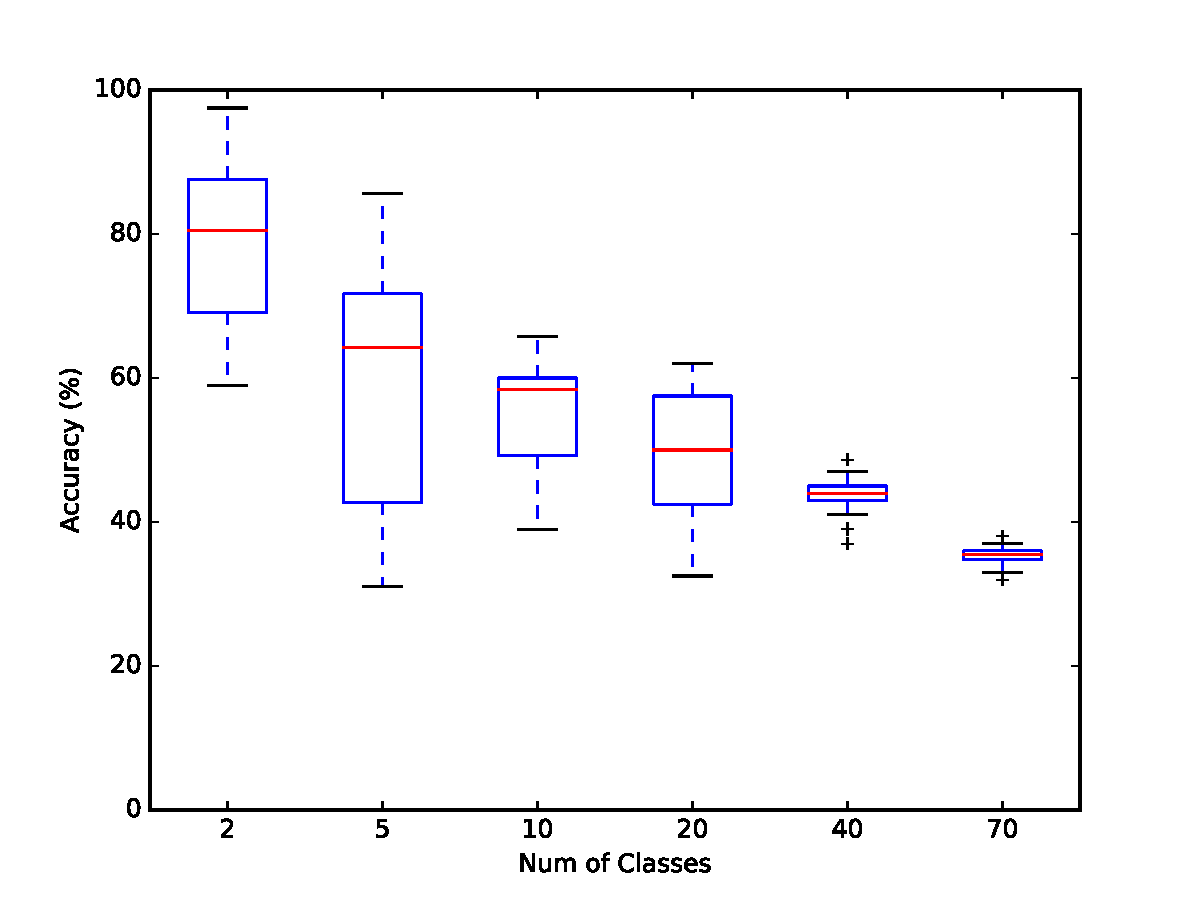
\includegraphics[scale=0.4]{specialization.ps}
  \caption{Box plot shows specialization effect. Accuracy are grouped by number of classes. Red line is the average accuracy for each given number of classes. The blue boxes stand for the 25\% and 75\% percentile accuracy. The black lines show the minimum and maximum accuracy.}
  \label{fig:specialization}
\end{figure}



\section{Class correlation}
\subsection{Impact on accuracy}
Runtime class distribution has been widely reported as having power in increasing accuracy and reducing energy (\cite{han2016mcdnn, kang2017noscope, shen2017fast}). The factor considered in existing papers about specialization is number of classes. It is believed that as we decrease number of classes, the accuracy would increase. Another belief is that the accuracy would keep similar once the number of classes is chosen, no matter which classes has been chosen. Based on these two belief, frameworks \cite{han2016mcdnn, kang2017noscope, shen2016fast} are built and benefits are gained. In these papers, the scheduling framework will select CNN models according to runtime distribution based on model metadata like accuracy and energy cost. Whether the metadata is precise enough is the key to success of the framework, especially the accuracy. In existing papers, the only factor considered is the number of classes. The only method of collecting accuracy for an architecture is to sample a subset of classes according to the desired number of classes. From our experiments on CIFAR100 \cite{krizhevsky2009learning}, we found that class effect is the important factor and the results without considering class effect is error-prone and hard to repeat.

Fig \ref{fig:specialization} shows the effect from \textit{class correlation} on accuracy, which cannot be ignored. The model has four convolutional layers and three fully connected layers, which is similar to the simplified model commonly used in existing frameworks. The experiment is done on CIFAR100 with 100 fine labels and 20 coarse labels. Each coarse label will have five fine labels, which compose a natural measurement of class correlation. For each specific number of classes, the choice of classes is randomly selected, the model architecture is unchanged and trained with the data corresponding to the chosen classes. Then the accuracy is generated by using trained model to predict the corresponding dataset generated from testing dataset. For each specific number of classes, this experiment is done for $100$ times and the accuracy is collected and presented by boxplot. In fig \ref{fig:specialization}, we shows the result when number of classes is $2, 5, 10, 20, 40, 70$, which should be representative. Red line is the average accuracy for each given number of classes. The blue boxes stand for the 25\%  and  75\%  percentile  accuracy. Previously, we have the broad idea that reducing number of classes can always lead to an increase in accuracy. While our result also supports this broad idea, two fatal shortage of this broad idea is found and an important direction to use specialization better is found.

The first important observation is that, contrary to our general feeling, decreasing number of classes does not necessarily indicate the increase in accuracy. What make problems worse is that even a negative result may appear when reducing number of classes. As we decrease the number of classes from $10$ to $5$, instead of increasing, the minimum accuracy decrease from 39.6\% to 31\%. Further, the minimum accuracy when the number of classes equals five is even much lower than the minimum accuracy when that number equals 70. The accuracy for a given number of classes varies, because the chosen classes varies in each sampling. Since we cannot control what classes will appear in the runtime, the claim that decreasing number of classes can increase accuracy does not hold, or only hold sometimes.

The second pivotal observation is that the variance of accuracy for a specific number of classes is huge, which makes it infeasible to use a single value as the representative for the performance of a model architecture on a specific number of class. When the number of classes is 2, the accuracy varies from 59\% to 98\%. In this case, the different of the maximum accuracy and minimum accuracy is almost 40\%. While 98\% is a good enough accuracy for arguing that use simple model to replace original full model, 59\% is such a bad result that no one wants to use the simple model, especially considering that the accuracy of random guess is 50\% in this case. However, in existing papers, a single value is used to represent the accuracy for a pair of model and number of classes. No one knows whether 59\% or 98\% is the value being used. And the dramatic variance of accuracy makes neither of them acceptable. From fig \ref{fig:specialization}, we can also find that the variance increases significantly as we decrease the number of classes. Considering that the specialization should be used when number of classes is much less than original number of classes, this observation makes the problem worse.

The reason behind the scene is the \textit{class correlation}. Some classes have strong correlation between each other and it would be extremely hard to classify them. When the number of classes is small, it is more probable that two or five similar classes are chosen simultaneously. When the number of classes is large, it is hard to only select the classes which are hard to classify and the classes that could be classified easily will make the accuracy higher. Thus small number of classes would be more prone to produce worst and best accuracy and give higher accuracy and large number of classes tends to produce similar accuracy and have low variance. 

\begin{table}[!th]
    \centering
    \begin{tabular}{|c|c|}
        \hline
    %    \multicolumn{1}{|c|c|} labels & Accuracy \\
    %    \hline
         Classes & Accuracy \\
         \hline
         (boy, girl) & 59.2\% \\
         (orchid, tulip) & 79.0\% \\
         (fox, pine) & 92.5\% \\
         \hline
        (baby, boy, girl, man, woman) &  31.49\% \\
        (clock, keyboard, mushroom, orange, pear) &  68.60\% \\
        (skyscraper, oranges, girl, bus, oak) & 84.6\% \\
        \hline
    \end{tabular}
    \vspace{1em}
    \caption{This table shows the interaction between class correlation and accuracy.  }
    \label{tab:classCorrelation}
\end{table}

To better support the importance of \textit{class correlation}, we look into detail about which groups of classes give low accuracy and give an intuitive explanation of \textit{class correlation}. Table \ref{tab:classCorrelation} shows the choice of classes and the corresponding accuracy. Setting the number of classes as two, the accuracy of classifying boy and girl is 59.2\%. If we try to classify fox and pine, the accuracy increase to 92.5\%, even if we have changed nothing in the model architecture. The only difference that could lead to this 33\% increase in accuracy is the chosen classes. Boy and girl shares more similarity than fox and pine. If we set the number of classes as 5, the accuracy of baby, boy, girl, man, woman is 31.49\% while the accuracy corresponding to skyscraper, oranges, girl, bus, oak is 84.6\%. This time, there are 53.11\% difference in accuracy. Intuitively, the difference between second groups of classes is much larger than the first group. Through experiments, we have proven that this similarity between classes plays an crucial role in testing accuracy. We call this similarity between classes as \textit{class correlation}.

\subsection{Metric: Semantic Tree}
Once have shown the importance of \textit{class correlation}, a metric to represent the similarity is desired and this metric will be used as the base for directed search, a mapping from classes input to suitable model, which will be discussed in section 3. Table \ref{tab:classCorrelation} shows that the similarity between natural language could be a good indicator of similarity between classes. From table \ref{tab:classCorrelation}, we can find that boy and girl have low accuracy while these two classes belong to the same coarse label: people. This observation also holds for orchid and tulip both belonging to flowers. In contrast, fox and pine belong to different coarse label and thus have much higher accuracy 92.5\%, while the other two groups only have 59.2\% and 79.0\% respectively. This observation also holds when there are five classes. Baby, boy, girl, man and woman have extremely low accuracy as 31.49\%, only slightly better than the accuracy of randomly gussing, which is 20\%. Again, these five classes have the same coarse label. If we choose classes from two coarse labels, the accuracy would increase dramatically. Clock, keyboard, mushroom, orange and pear are five labels from two coarse labels: electrical devices and fruit. The accuracy for these classes would increase to 68.6\%. The accuracy would increase further, if we choose classes from five different coarse labels. Skyscraper, oranges, girl, bus and oak comes from five different labels and the accuracy is 84.6\%, which is much higher than previous two groups. Based these observations, we find \textit{semantic tree} is a good metric for class correlation, which measures the similarity between concepts from the perspective of human language.

\begin{figure}
\centering
  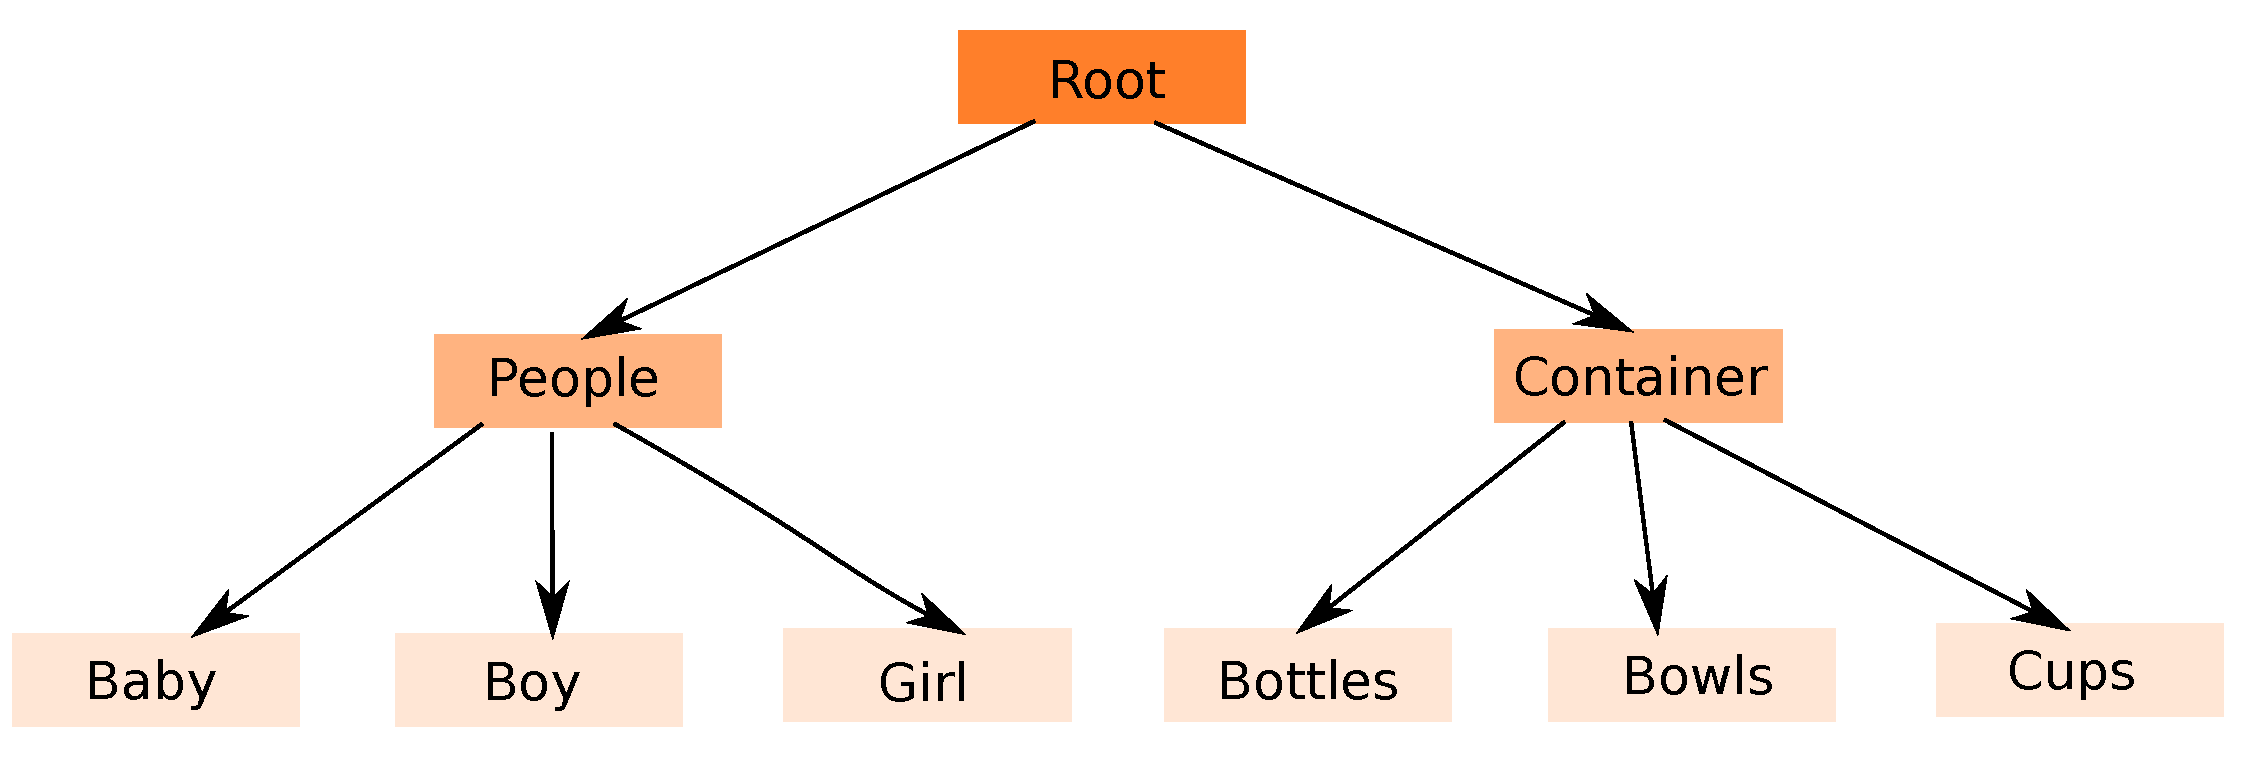
\includegraphics[scale=0.2]{semanticTree.ps}
\caption{An example of semantic tree generated from CIFAR100}
\label{fig:semanticTree}
\end{figure}

%给出tree的定义和使用例子。
\textit{Semantic tree} is a  tree-structured storage of images, widely used to organize images. In CIFAR100, there are 20 coarse labels and five fine labels under each coarse label. $2500$ images are labelled by each coarse label and each fine label contains $500$ images. Thus there is a hierarchy structure organizing images naturally. ImageNet  \cite{deng2009imagenet, imagenet_cvpr09} also organizes images in a tree-structured way. Thus semantic tree is widely existed in various large dataset and could be easily accessed. In a tree-structured storage, images will be grouped by labels and labels will be indexed like a tree according to their similarity in semantics. For example, the root might be mammal and has two children: dog and cat. Under the cat node, there are some children and each children node represents a cat species. Fig \ref{fig:semanticTree} shows a part of semantic tree in CIFAR100. The second layer contains coarse labels and the third layer contains fine labels. For example, "people" is a coarse label, and the 5 corresponding fine lables are "baby, boy, girl, man and woman" from "people" label. Thus "people" is the child of root and "baby, boy, girl" are the children of "people" node.  If two images belongs to different coarse labels, we say that there is low class correlation between these two images. For images with the same coarse label but different fine labels, they are said to have high class correlation. If two images have the same fine label, they are indistinguishable from the point view of prediction. In CIFAR100, we can define the similarity of a groups of classes as 
\begin{equation}
    \frac{1}{|\{ CL_1  \} \cup \{ CL_2\} \cup \cdot \cdot \cdot  \cup  \{ CL_n\}  |}
\end{equation}
,
where CL means coarse label and $CL_i$ means the coarse label corresponding to the $i$th entry. The intuition of this value is that classes from same coarse label are treated as similar and as more classes come from the same coarse label, the class correlation will increase and the metric will also increase. Thus the larger the metric is, the more correlation selected classes have.

%用tree证明之前的结论
\begin{figure}
\centering
  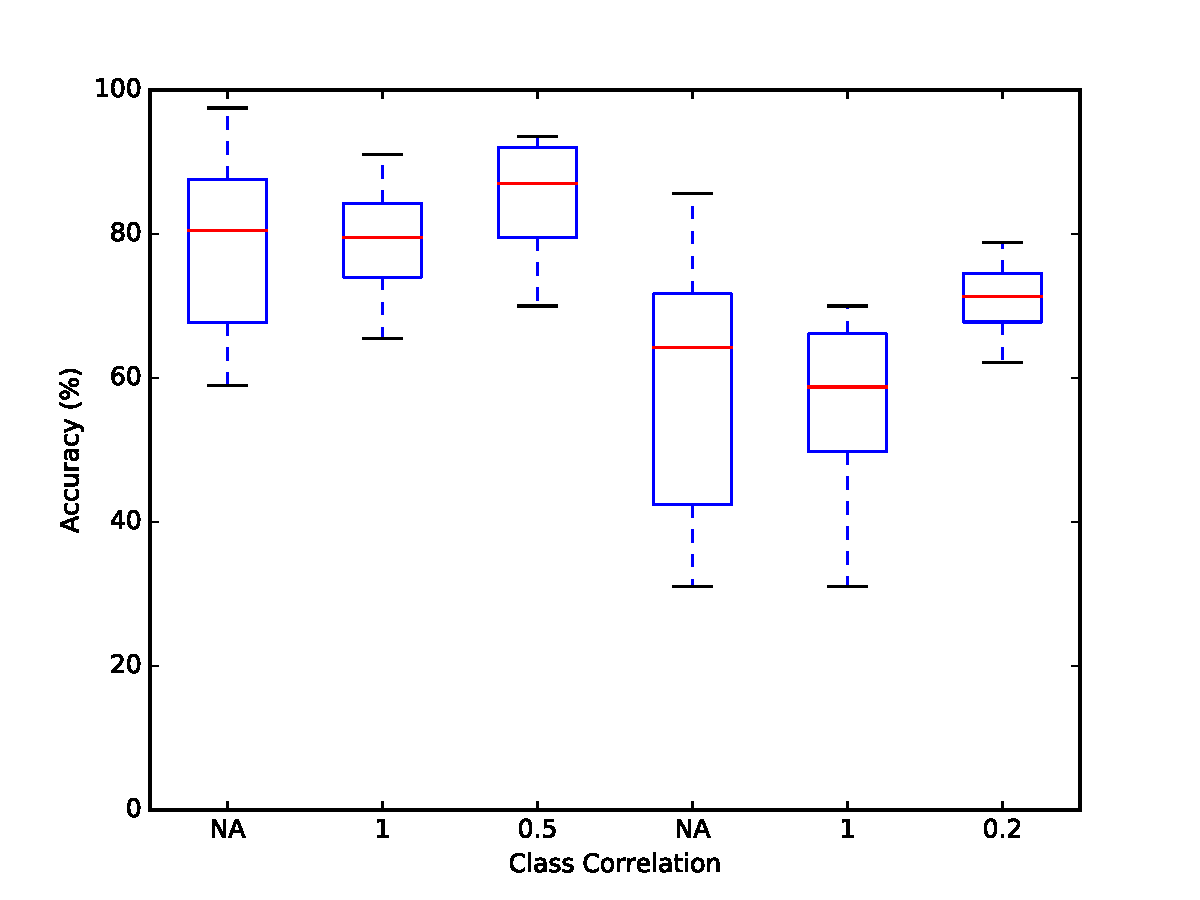
\includegraphics[scale=0.4]{metricTreeEffect.ps}
\caption{Showing the boxplot of accuracy grouped by class correlation. The first three is the boxplot for class number equals 2. The second three are the boxplots when class number equlas 5. NA means the accuracy when we do not consider class correlation. Numbers are the class correlations calculated following the definition of metric tree. }
\label{fig:semanticTreeEffect}
\end{figure}

Semantic tree is powerful in predicting the testing accuracy. Using the same model, classifying classes close to each other in semantic tree tends to have low accuracy while high accuracy often comes with classes far from each other in the semantic tree. The accuracy is $75\%$ when we use Model1 to predict from 5 coarse labels: quatic mammals, flowers, household furniture, insects, and people. In contrast, if we use finer labels inside each of these coarse labels, like "baby, boy, girl, man and woman" from "people" label, or "beaver, dolphin, otter, seal, whale" from "aquatic mammals" label, the accuracy would decrease dramatically to $55\%$, even if we have changed nothing with number of classes in the softmax layer and the model architecture. This result shows that semantic tree has certain power in predicting accuracy: classes with high similarity gets low accuracy and classes with low similarity gets high accuracy.

Fig \ref{fig:semanticTreeEffect} shows the benefit gained by semantic tree from a statistical perspective. The first three box plots are for two classes and the second three box plots are the accuracy when number of classes is 5. NA stands for the case when we do not use semantic tree. The numbers on x axis are the class correlation calculated by the formula mentioned before. When number of classes is 2, without considering class correlation, the accuracy ranges from 59\% to 97\%, where the difference is 38\%. If the class correlation is 1, which means strong class correlation, the accuracy would range from 66\% to 90\%, where the difference decreases to 24\%. When the class correlation is 0.5, the accuracy would range from 70\% to 90\%, where the difference decrease to 20\%. When number of classes is 5, without considering class correlation, the accuracy ranges from 31\% to 85\%. In this case, the difference between minimum accuracy and maximum accuracy is 54\%, which is extremely huge. After considering class correlation, this difference decrease to 39\% and 13\%, for class correlation equals to 1 and 0.2 respectively. Thus considering both number of classes and class correlation would decrease the variance of accuracy and make the metadata used in scheduling model more trustable.

\section{Guided search: Mapping from Classes to Model}
Through using runtime distribution and a series optimization methods, we will have a trade-off between accuracy and energy. These two parameters will be measured in advance and compose the base for runtime decision by the scheduling model \textit{SMART}. \textit{SMART} will take into consideration the remaining energy, desired accuracy, and pre-collected model accuracy. The intuition of \textit{SMART} is to use a complex enough model such that the pre-collected accuracy for that model can match the target while the selected model are not too complex to cost too much energy. In this case, the precision of metadata becomes critical for the efficient runtime decision. If the variance of accuracy for a model on different groups of classes is too large, we cannot use a single number to represent the model accurac, which results the instability of the whole framework performance.

In existing papers \cite{han2016mcdnn, shen2016fast, kang2017noscope}, the framework for storing metadata and supporting runtime decision can be summarized in two equations. In storage, the metadata is organized in the following format 
\begin{equation}
    (model, numberClasses) \Longrightarrow accuracy,
\end{equation}
while in runtime, the information is retrieved by the following function
\begin{equation}
    model = f(target, numberClasses)
\end{equation}
, where target is the desired accuracy. As we have demonstrated in section 3, previous framework does not consider class correlation and, for a given model and number of classes, the difference between maximum and minimum accuracy could be as large as 50\%. Thus the representative ability of this framework is very limited. 

To give a more precise metadata, we must take the class correlation into consideration. The main obstacle is that, for a given number of classes, the combination of classes is mind-bogglingly huge. For example, if we have 100 classes in total, the number of possible combinations is $100!$. It is entirely impossible to measure and record their accuracy one by one. Our solution is to use class correlation. We will first use metric tree to calculate a digit to represent the class correlation between selected classes. Then groups of classes with that class correlation will be sampled for 100 times and the accuracy for these groups are tested. After the experiments, we will collect the average accuracy and the difference between the maximum accuracy and minimum accuracy for each class correlation digits. In summary, the metadata will be organized in the format
\begin{equation}
    (model, numberClasses, metric) \Longrightarrow accuracy,
\end{equation}
in the preparation period and in the runtime we will query the databse for metadata by
\begin{equation}
    model = f(target, numberClasses, metric).
\end{equation}

This method will perform better than previous work since variance will decrease dramatically after we divide groups of classes by class correlation. One shortage is that sometimes the difference between maximum and minimum accuracy is still larger than 20\% which makes the metadata not so trustable. To ease this problem, we will use 25-percentile accuracy, instead of accuracy, to represent the testing accuracy when the difference is larger than 20\%. Through this way, we can have strong confidence that in more than 75\% runs the selected model will perform at least not worse than the target accuracy. This is a system design choice favoring accuracy over energy. This design choice will force the framework accuracy better than user's expectation on accuracy. The overhead introduced by the design choice will be made up by scheduling model through considering many other models when possible, since different model will have various difference between maximum and minimum accuracy for a given number of classes and class correlation. To match this design choice, the storage and query format should also be modified appropriately as
\begin{equation}
    \begin{split}
        (model, number&Classes, metric) \\
            & \Longrightarrow adjusted\_accuracy,
    \end{split}
\end{equation}
for storage and
\begin{equation}
    model = f(target, numberClasses, metric)
\end{equation}
for query.

\section{Optimization Methods}
The improvement in accuracy brought in by class skew provides the space for model simplification. In other words, even if we simplify a model dramatically and use much less resource, we can still achieve a similar accuracy with the original full model. Existing model optimization methods (Reference TO BE ADDED) does not make use of the class skew and cannot exploit thoroughly the space introduced by class skew. Thus we explore a series of class-skew related optimization methods, including number of nodes in softmax layer, number of layers, distillation, and reducing input size. 

\subsection{Reducing number of nodes in the softmax layer}
Number of nodes in the softmax layer represents number of classes that we want to predict from. When less number of classes appears in an environment, a natural change in the CNN architecture is to reduce number of nodes in the softmax layer. The benefits are two fold. First, reducing number of classes can increase testing accuracy. If we randomly guess from 1000 classes, the expected accuracy would be $0.1\%$. The expected accuracy for random guess would increase to $50\%$ if there are only 2 classes. This observation also holds for CNN models. Second, reducing number of classes can decrease memory usage. In VGG16 \cite{simonyan2014very}, 89.36\% parameters exist in the fully connected layer. Reducing nodes in the softmax layer can reduce parameters proportionally and use less memory. A point worth noting is that most of computation exists in the convolutional layers. Thus reducing nodes in the softmax layer cannot save computation and power. This task is generally achieved by other optimizations.

\subsection{Reduce number of layers}
Reducing number of layers is a prevalent methods in specialization, which has benefit in reducing computation and shortage in decreasing accuracy. Reducing number of layers, especially the convolutional layers, is a good method in reducing computation. Taking VGG16 for example again, $99.20\%$ computations exist in convolutional layers and spreads evenly across all the convolutional layers. Thus reducing number of layers can reduce computation proportionally. The negative side is the decreas of accuracy. Less layers means a shallower network which has been reported \cite{han2016mcdnn, shen2017fast} to have worse performance than deep models. However, this decrease in accuracy is made up by the increase introduced by reducing number of nodes in softmax layer. Thus these two methods together can decrease energy and increase accuracy, which is the key for the benefit claimed in previous papers.


\subsection{Distillation}
Distillation \cite{hinton2015distilling} is a method that can contribute to the model specialization and has not been introduced into specialization. The idea of distillation is using a deep model to train a shallow model. Deep models with higher accuracy would contain more information than shallower models. When we train the shallow model, we can treat the deep model as teacher and the shallow model as student. Instead of train the student model directly on the original datasets with a vector of only 0-1, we can train the student model to mimic the logits of large model, which indicates how strongly the teacher model believes that this image belongs to this specific class. In this way, the student model can learn more information from the teacher and achieve a higher accuracy. 

Original paper \cite{hinton2015distilling} assumes that the number of classes in the shallow model is same as the number of classes in the deep model. This does not hold in specialization. In distillation for specialization, we will simply truncate the output of softmax layer and only use the output corresponding to the observed classes.

\subsection{Input Size}
Reducing input size is another method that exists in other areas and has not been introduced into specialization \cite{krizhevsky2009learning, fu2017look}. Input size has influence on resource computation and model accuracy. With the same model on CIFAR100, if we reduce the input size from 32*32 to 16*16 and further to 8*8, the accuracy will only decrease from 25\% to 23\% to 21\%, in the mean time the computation and memory cost has decreased by 4 and 16 times, respectively. Thus we can treat input size as a hyper-parameter and fine-tune this parameter according to available resource and targeted accuracy. In the training period,  we need to downsample the training dataset into a smaller resolution and train the model on this down-sampled dataset. In the reference period, the input image should also be down-sampled to the same resolution. In this way, we can get significant benefit in energy efficiency while only lose little on accuracy.



\section{Important factor in real life usage: Retrain}
To use runtime class distribution, retraining is required since originally we only have a full model targeting thousands of classes. We cannot pre-train models for all possible combination of classes due to two reasons. First, we cannot predict the runtime class distribution before we actually see it. Second, the total combination of classes is a mind-boggling number such that it is unfeasible to pre-train models for each of the combination. Since the resource consumption by retraining is huge, methods for avoid retraining the whole network is desirable. We will discuss the shortage of method used by existing papers first and then bring up two innovative methods to avoid runtime retraining.


\subsection{Retrain last few layers}
The only existing methods for solving retraining problem is to retrain the last few layers, widely used in specialization \cite{han2016mcdnn, kang2017noscope, shen2017fast} and transfer learning \cite{razavian2014cnn, zhuang2015supervised, sun2016return}. In this method, only the last few layers will be retrained. Parameters of preceding layers will be kept and architecture will remain unchanged. There is no strict standards to determine how many layers should be retrained or predict the accuracy for the choice. Literature reports that more layers are retrained, more benefit on accuracy is gained. 

There are both good and bad sides for this method. Good side is that retrained model can still make use of features learned by leading layers and retraining from scratch can be avoided. The bad sides are the energy constrain and time latency. In the retraining process, hundreds of images need to go through the network for several rounds. In the resource constrained environment, this is a unbearable waste of energy. Without this waste, the device can process tens of thousand images and give user better endurance. Further, the time latency is also annoying even if the device has sufficient energy. The shortest retraining time reported by \cite{shen2016fast} is four seconds. Compared to network latency measured in milliseconds, four seconds latency is too long to be accepted and will deteriorate user experience dramatically. To solve both the energy wasting problem and long latency problem, we will bring up \textit{cold retraining} and \textit{probability layer} to supplement or even replace retraining last few layers.

\subsection{Repeated patterns in daily life and cold retrain}
In daily life, same environment and class distribution will appear again and again. Our family members are fixed for tens of years. In office, we will stay in the same company for at least several months and the collaborators are generally fixed. In films like \textit{The Big Bang Theory}, characters are also fixed. Using this repeated pattern, we do not need to retrain models every time. We can retrain the model once and use that model for all similar environment afterwards. Actually we even do not need to retrain the model in the runtime. In the first time we confront a new scenario, we can record the distribution on disk and use \textit{probability layer} described in the next subsection to be the runtime cold-start. When the users go back home and connect the mobile device to power and WiFi, we can cold retrain the model to whatever extent without worrying about the energy and memory limit, which would give us more benefit on accuracy.

%\textit{Experiments: use Youtube videos to show repeated patterns in daily life}



\subsection{Probability Layer}
\textit{Probability layer} is an extra layer after the softmax layer in the CNN models. With \textit{probability layer}, we can use runtime class distribution without retraining. As we have discussed previously, there are gains in both reducing energy consumption and time latency. Existing methods, i.e. retraining last few layers, requires thousands of images to go through the network for tens of rounds, which waste lots of energy. The retraining also takes time and introduce several seconds latency during which new images cannot be processed. With \textit{probability layer}, all of these inconvenience will be avoided and better performance will be gained. Thus \textit{probability layer} is a brilliant supplement or even replacement of retraining last few layers.

To implement probability layer, the only thing we need to do is to add an extra layer after the softmax layer. Originally, the last layer of CNN model is softmax layer. The output of softmax layer is a vector $(p_1, p_2, ..., p_n)$, where $n$ is the number of nodes in the softmax layer, i.e. the number of classes that the CNN model wants to predict from. Also, $p_1$, ..., $p_n$ is a series of numbers between $0$nd $1$. Thus we would treat $p_i$ as the probability that indicates how likely an image may belong to a specific class $i$. The main idea of probability layer is to add a constant to classes that is more likely to be the true label according to the runtime distribution. For example, if the runtime distribution shows that only the first 10 out of 100 classes could appear in a context, the probability layer will add a constant to $p_1$, ..., $p_{10}$, the predicted probability of these 10 classes. In other word, in this case, the probability layer is $ c_1, c_2, c_3, c_4, c_5, c_6, c_7, c_8, c_9, c_{10}, 0, ...,0 )$, where $c_i$ is a constant between $0$ and $1$ and the output of the probability layer is $(p_1 + c_1, p_2 + c_2, ..., p_{10}+c_{10}, p_{11}, ..., p_{100})$. Here we treat $c_i$ as hyper-parameters. The larger the $c_i$ is, the stronger confidence we have in runtime distribution.

The success of probability layer depends on the accuracy of original model. Intuitively, adding a constant to a set of domain classes according to the run-time distribution would encourage the model to select among these domain classes. If the original model is precise, i.e. have high top-5 accuracy, this constrain could rule out some classes and help the model to get a correct result. For example, if the output of softmax layer is $(0.3, 0, ..., 0, 0.7)$ and the probability layer according to runtime distribution is $(0.5, 0.5, 0.5, 0.5, 0.5, 0, ..., 0)$, the output of probability layer would be $(0.8, 0.5, 0.5, 0.5, 0.5, 0, ..., 0.7)$. Assume the correct label is $0$,  the prediction without probability layer is $99$, which is wrong, and the prediction with probability layer is $0$, which is correct. In this case, probability layer helps us to rule out the unlikely class $99$.

A possible case is that the probability corresponding to the true label are not highest even in domain classes. In this case, the probability will not be helpful. We found that top-5 accuracy is a good meric to measure how well the probability layer could help the original model. In other word, the benefit of probability layer is to improve the top-1 accuracy to be as large as the top-5 accuracy. If the top-5 accuracy is very high, the true label would have the top-5 high probability. The probability layer will constrain the predicted label to be the intersection between these top-5 labels and the domain labels according to runtime distribution. Thus we can increase top-1 accuracy toward top-5 accuracy. 

However, if the number of domain classes are 5 and the top-5 accuracy of the model is low, it is possible that the probability of true label is not the highest among the 5 domain classes. In this case, the benefit of probability layer would be slight. Thus, the higher top-5 accuracy the original model have, the better effect the probability layer would bring. In other word, if we use probability layer on a model with low top-5 accuracy, the benefit would be small. 





\subsection{Comparison with naive mask}
A naive replacement of \textit{probability layer} is to mask all non-domain classes, called \textit{naive mask}. Probability layer is a generalization of naive mask. In fact, naive mask is equivalent to set the parameter $c$ in probability layer to be $1.0$. The intuitive explanation of naive mask is to only have nodes according to the main classes since the predicted label could only be one of these domain classes. If we use naive mask, all the prediction of images with classes besides the main classes would be wrong. This would limit the usage of naive mask dramatically. For example, if the domain classes occupy 70\% in the runtime distribution, the accuracy with naive mask would be less than 70\%, which is smaller than the accuracy without naive mask and makes naive mask useless, even if 70\% skew is not a low skew in daily life. 

Probability layer can avoid this problem if we set the parameter c to be strictly less than 1.0. This benefit depends on high accuracy of original model again. Generally, in denseNet \cite{huang2017densely}, if an image could be classified correctly, the probability corresponding to the correct label after softmax layer is 1, and the probability corresponding to other labels are almost 0. For example, if the true label of an image is $11$, the output of softmax would generally be $(0, 0, 0, 0, 0, 0, 0, 0, 0, 0, 1, 0, 0, 0, 0, ... 0)$. Even if we add a probability layer to first 10 classes and use the parameter as 0.9, the output would be $(0.9, 0.9, 0.9, 0.9, 0.9, 0.9, 0.9, 0.9, 0.9, 0.9, 1, 0, 0, 0, 0, ... 0)$. In this case, the model would still mark $11$ as the correct label and the probability layer has no bad effect. However, if we use naive mask to rule out all classes other than first ten classes, the prediction would be constrained in the first ten classes and will be wrong. 

In other words, the probability layer only has bad effect when the original model is not quite sure about how to classify an image. For example, if the true label of an image is 11, the output might be $(0.3, 0, 0, 0, 0, 0, 0, 0, 0, 0, 0.7, 0, 0, 0, 0, ... 0)$. After we add the probability layer to first 10 classes and use the parameter as 0.9, the output would be $(1.2, 0.9, 0.9, 0.9, 0.9, 0.9, 0.9, 0.9, 0.9, 0.9, 0.7, 0, 0, 0, 0, ... 0)$. In this case, the model would mark 1 as the correct label and the probability layer have a bad effect. However, the happen of this bad effect needs two conditions. First, the labels with predicted probability 0.3 and 0.7 also appear in the first ten classes. Second, the predicted probability of true label is lower than the other one. Actually this is a rare case.


\section{Architecture}
In this section, we will describe the architecture in detail. Figure \ref{fig:Architecture} gives an overview of the architecture. Basically, we have 5 parts including two storage parts, class catalog and model store, one scheduler, one executor, and a profiler. The storage components, class catalog and model store, are used for saving metadata and providing supporting information for decision. The scheduler is a scheduling model to decide the choice of models in the runtime according to available resource and demanded accuracy. The target of the scheduler is to maximize the accuracy while adjust the energy consumption automatically according to remaining energy. The scheduler will also have a have high-accuracy mode just in case that users confront important scenario and want to get the best accuracy no matter how much energy the model will cost, or the user knows that a re-charge will be available soon. Once the scheduler made a decision, the executor will execute the model and the profiler will record the predicted value and update its record for future reference from the scheduler. Now we will discuss each component in detail.

\subsection{Profiler}
For every image, there would be a CNN model to classify it, either a full model or a specialized model. Thus every incoming image will have a predicted label. The profiler will record the distribution of classes and report the class skew to the scheduling model, which will use this information to choose the model. There would be two behaviors of profiler. First, the profiler will report the class skew every minute. Generally, the class skew would keep similar and change gradually as time goes and the class skew in current minute is a good approximation of the class skew in the following minute. And one minute is not a too short time period and hopefully a one-minute time window could see all the type of figures in current environment. This choice is a parameter instead of an unchangeable assumption. Second, after the profiler report the class skew to scheduler, it will still record the class skew. Through this way, the profiler can know, for this specific user, what kind of class skew will appear, how long the class skew will last, and how often this class skew will appear. This could be an important supporting information for the scheduler. If a class skew appears frequently, we can cold-retrain a complex model and save the model on disk. Once we see the class skew again, we can use this on-disk specialized model directly without retraining. Actually, it is quite common for a specific user that the same class skew appears everyday. For example, the people in family always remain same; the researchers will go to the lab everyday and the people in lab generally is changed once per year; the type and location of fitness equipments in a gym will also be same day by day. Once the profiler can detect this kind of class skew, the cold-retrain complex model could become a feasible choice.

\subsection{Class catalog}
When the profiler detect a class skew, we will consider not only the number of classes, but also the relationship between these classes. Class catalog is a tree-structured dictionary to group similar classes together. As we have discussed in section 2.2, if the detected class skew is close to each other in class catalog, it would be hard to classify these classes and the scheduler will use a more complex model to achieve the demanded accuracy. 


\subsection{Model Store}
In the beginning, there would be a collection of models without consideration on class skew. These models are for different purpose and with different degree of optimization. In the running time, as the profiler detect the class skew and usage pattern for the specific user, more specialized model, either hot retrained or cold retrained model, will be incorporated into the model store. When the device is connected to power and computation resource is enough, each model will be run on a benchmark, a collection of common datasets, like CIFAR100, and the average accuracy, energy and memory consumption will be recorded. In the run time, the scheduler can read this metadata from model store and use these information for decision. 

Another task that model store will accomplish automatically is to get the most efficient model for every energy budget. Given a energy budget, only the model with highest accuracy will be kept. In the same time, only the model with lowest resource consumption will be kept given a accuracy. This can be done by model store automatically since it is straightforward to calculate the number of parameter and computations just by going through a model without actually running. In this way, only the model that achieves Pareto optimality will be kept in model store and the scheduler can easily choose the most suitable model according to current energy budget just like a hash function.


\subsection{Scheduling Model}
The task of scheduling model is to select a series of models to process the image stream under a resource constrain. The target is to maximize the accuracy while try to use less energy for each image. The choice is between a cascades of models with different accuracy and different energy consumption. To solve this optimization problem, we build a heuristic algorithm, in Algorithm 1 and Algorithm 2 to allocate energy for each input image, choose the most suitable model given the per frame energy, and wrap all the decisions automatically.


Through a series of experiments (TO BE ADDED) on real-life videos, we found that the contents of a video would almost remain same in a single second, a process rate of one frame per second is enough for detect objects in the video. For energy efficiency consideration, we will use this configuration and estimate the per frame energy based on this observation. In concrete, $AllocateEnergy$ (line 11) will retrieve the expected running time and estimate per frame energy by averaging the available energy over all remaining time. In this case, saving energy in each frame still makes sense, since the saved energy will be allocated to future inputs and increase the accuracy of these inputs.

For giving more freedom to users, a $mode$ option is given through $scheduler$ (line 1) function. This option is useful if the user feel that current scenario is very important such that we want to sacrifice energy-efficiency for exchanging higher accuracy. In this case, the scheduler will expect to run for at least 10 minutes, no matter how long the original settled remaining time is, and allocate more energy to each frame. 



\begin{algorithm}
 \caption{Scheduling Model}
  \begin{algorithmic}[1]
    \Function{Scheduler}{$i, r, mode$}
        \Comment{i is the input image, r is the report from profiler about current class skew, mode is the user preference, target indicates the desired accuracy if mode is set to be EFFICIENCY}
        \State $AE = RemainEnergy()$    
        \Comment{AE stands for available energy}
        \If {mode == HIGHACCURACY}
            \State $PFE = AE / 600 $ 
            \Comment{PFE stands for perFrameEnergy, which is the energy allocated for every frame.}
        \ElsIf {mode == EFFICIENCY}
                \State $PFE = allocateEnergy(AE)$
        \EndIf
            \State $a, m = chooseModel(PFE, r)$  
                \Comment{chooseModel(PFE,r) is a function to access the metadata from class catalog and model store to decide the best accuracy we can achieve under current energy constrain and which model we should use}
            \State $execute(i,m)$        
                \Comment{execute(i,m) will retrieve the model m from model store and process the input image i with model m}
    \EndFunction

    \Function{allocateEnergy}{$AE$}
    \Comment{allocateEnergy(AE) allocates per frame energy according to current avalable energy and class skew}
        \State $n = RemainingTime()$    \Comment{remainingTime() will give the expected time to keep running. We will process one image per seconds and n is the remaining time in second as well as the expected number of images to classify.}
        \State $PFE = AE/n$
        \State \Return $PFE$
    \EndFunction
        \Function{chooseModel}{$PFE, r$}
        \If{$Parse(r) == NoSkew$}
            \State $a, m = getModel(PFE)$   \Comment{If there is no class skew, getModel(PFE) will return the model with highest accuracy given the per frame energy budget PFE}
        \ElsIf{$Parse(r) == Skew$}
            \State $a,m = ExistedRetrainedModel(r, PFE)$
            \If{$m == NULL$}
                \If{$PFE > \Delta E/600 + FrameCost(m,r)$}
                    \State $a,m = retrain(m,r)$
                \Else
                    \State $a,m = probabilityLayer(m,r)$
                \EndIf
            \EndIf
        \EndIf
        
        \State \Return $a,m$
    \EndFunction

    
\end{algorithmic}
\end{algorithm}

\begin{figure*}
\centering
\begin{subfigure}{.5\textwidth}
  \centering
  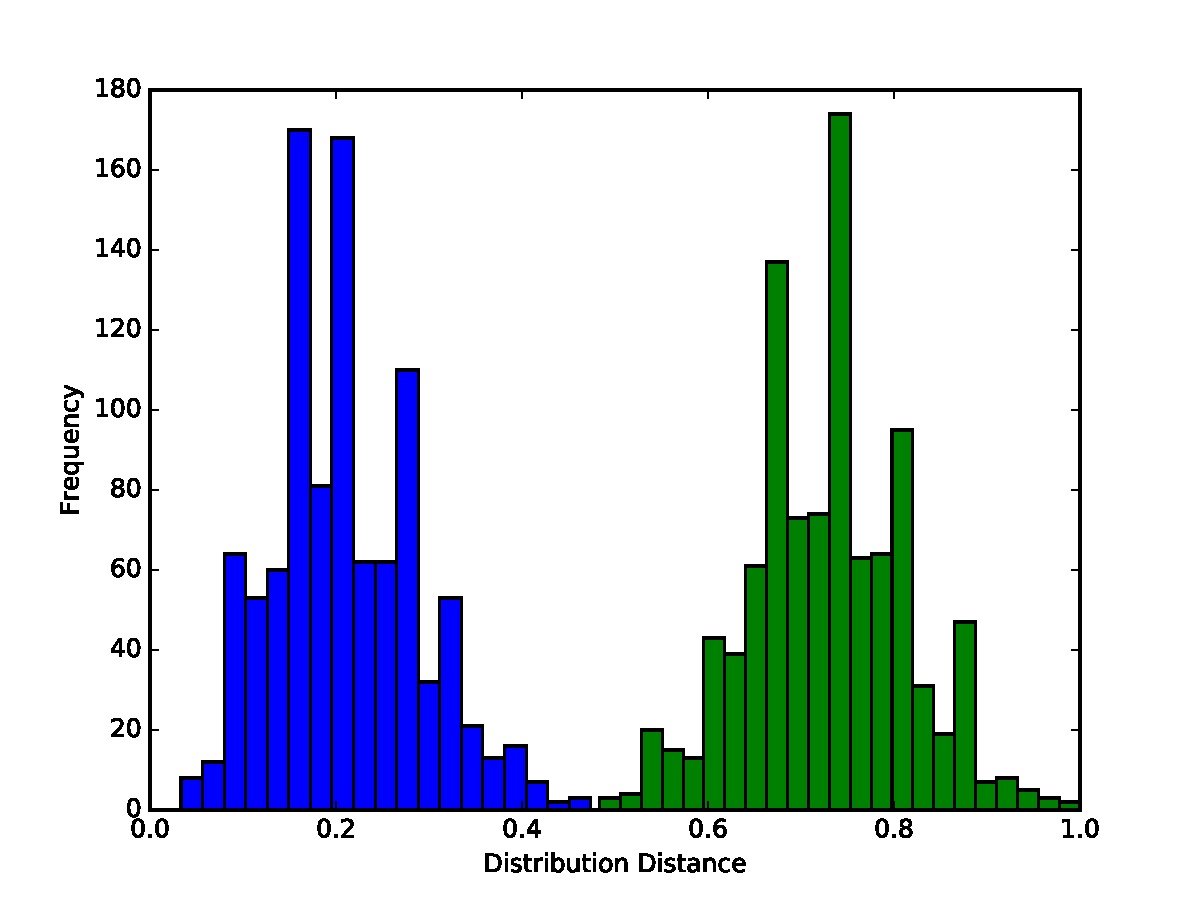
\includegraphics[scale=0.4]{profiler1.ps}
  \caption{Four classes overlapping}
  \label{fig:distributionDistance1}
\end{subfigure}%
\begin{subfigure}{.5\textwidth}
  \centering
  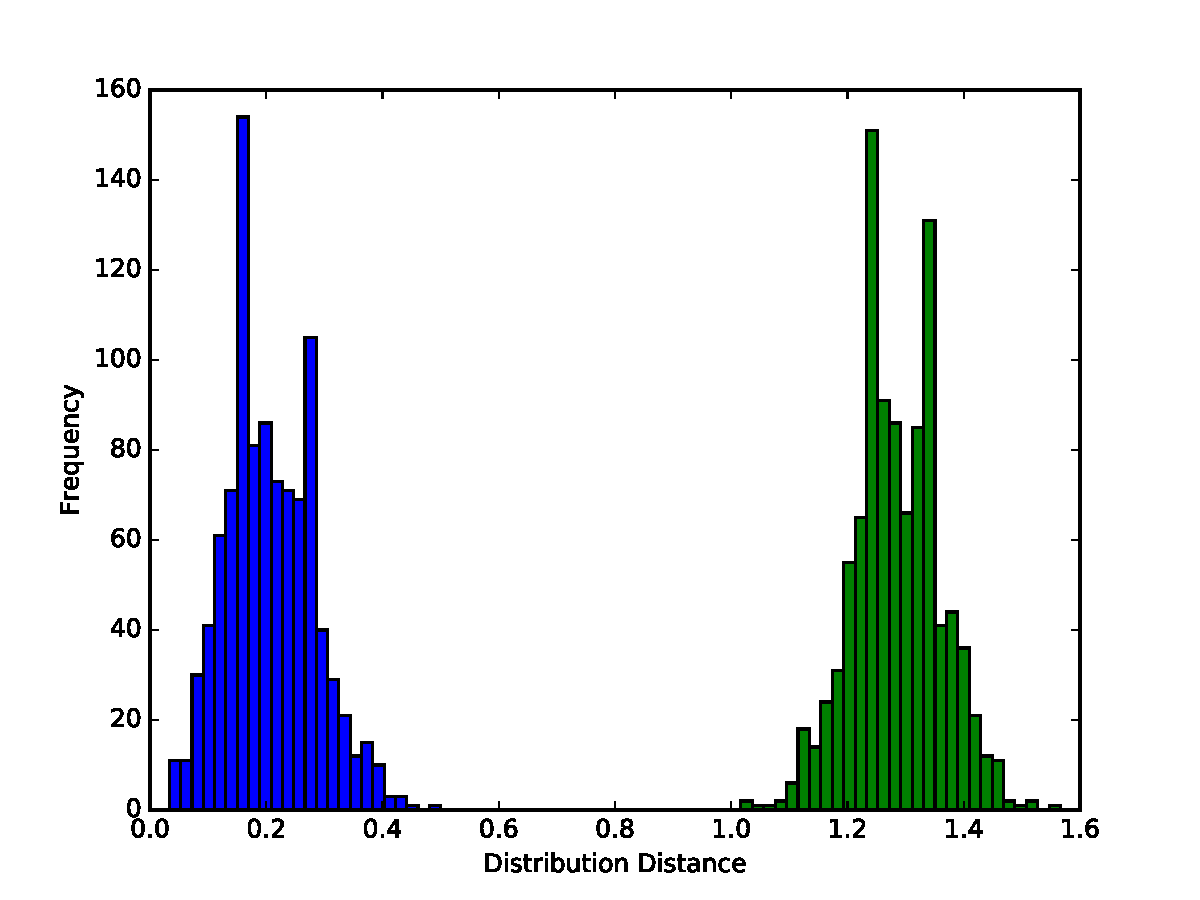
\includegraphics[scale=0.4]{profiler2.ps}
  \caption{Two classes overlapping}
  \label{fig:distributionDistance2}
\end{subfigure}

\caption{Graphs showing the distance between data distribution of two classes groups}
\label{fig:distributionDistance}
\end{figure*}

Given per frame energy budget and recorded class skew, $ChooseModel$ will return the best model. If no class skew exists, $ChooseModel$ do not need to consider retraining and will choose the model with highest accuracy given current energy budget. When there is class skew, the $ExistedRetrainedModel$ will check whether there are retrained model for current class skew and return a suitable model. When there is no retrained model on disk, the architecture will choose between retraining last few layers and using probability layer. Since retraining is costly, we expect to have enough energy to run that retrained model for at least 10 minutes, otherwise it is more feasible to avoid retraining and use probability layer directly.


The scheduler will wrap up all the algorithms in scheduling model and give the most suitable model. For every input image $i$, The scheduler needs to get the class skew report $r$ from profiler. In the high accuracy mode, enough energy is given to each image such that more freedom in choice of models is allowed. In the efficiency mode, $allocateEnergy$ will estimate per frame energy according to expected remaining running time. Given this per frame energy and class skew report, the chooseModel will give the best model $m$ and the corresponding accuracy $a$. Finnaly, the $scheduler$ will call $execute(i,m)$ to run the model $m$ on input image $i$.


\section{Experiments}
\subsection{Detection overhead}
The fundamental of using runtime distribution is detecting runtime distribution, mainly focused on the number of classes and what classes are appearing. Profiler is the component in \textit{SMART} taking care of this detection. As images come, full models will classify these images and profiler will store the results. For every $120$ processed images, the profiler will calculate the distribution of these classified images and compare with the distribution for last $120$ images. We choose $120$ because generally we will process $1$ image per seconds and $120$ images will represent the distribution of classes in two minutes. Assuming there are $n$ classes in the full model, the frequency of each class will be recorded as $f_i$, which is the proportion that this class appears. The profiler will calculate the difference between two distributions by 
\begin{equation}
    distance = \sum_{i = 1}^{n}(f_i^1 - f_i^2)
\end{equation}
, where $f_i^1$ is the frequency of class $i$ in the first distribution and $f_i^2$ is the frequency of class $i$ in the second distribution. If the distance is less than $0.5$, we will claim that distribution has been stabilized and a runtime distribution has been detected. Fig \ref{fig:distributionDistance} shows profiler performance. In fig \ref{fig:distributionDistance1}, the blue histogram is the distribution of distance when all images are selected from class $0$ to $4$ and the green histogram is the distribution of distance when images comes from classes $0$ to $4$ and $1$ to $5$ alternately. If the distance between two distribution is less than $0.4$, we can assert that classes in these two consecutive time period are same. In fig \ref{fig:distributionDistance2}, the meaning of blue and green histogram are same as in fig \ref{fig:distributionDistance1}. The only difference is that the groups of classes in fig \ref{fig:distributionDistance2} is $0$ to $4$ and $3$ to $7$, where class groups have less overlap than fig \ref{fig:distributionDistance1}. In this case, the distance between two histograms larger. As we decrease the overlap further, the distance between two histograms will become larger. Thus the choice of $0.4$ as detection criterion works. Based on these experiments, four minutes or $240$ images would be enough for detecting runtime class distribution.








\subsection{Probability Layer}
A series of experiments on various kind of specialized datasets have shown the effectiveness of probability layer. CIFAR100 is a prevalent benchmark for various kind of CNN models, which has 100 classes, a training dataset with 500 images per class, and a testing dataset with 100 images per class. To mimic the runtime distribution, we generate a specialized dataset manually. For example, in generation of a specialized dataset with 80\% data skew and 10 domain classes, we would use 1000 images from the testing dataset according to these 10 domain classes, and randomly select 250 images from other classes. We trained the model on original CIFAR100 training dataset and test the model on various kind of specialized datasets with different number of domain classes and selection of domain classes. We also take into account that the selection of domain classes because the choice of labels have strong effect on the test accuracy, even if we keep the number of domain classes unchanged. Actually some classes are easier to classify than others. To eliminate this random effect, we will choose different groups of labels for each number of domain classes.

Figure \ref{fig:ProbabilityLayer} summarizes the results. As a benchmark, the test accuracy on the CIFAR100 testing dataset without probability layer is 73.74\%. If the number of domain classes is 2 and we choose the label 0 and 1, the accuracy without probability layer is 88.12\%. The difference between specialized testing accuracy 88.12\% and the overall accuracy 73.74\% is due to selection of classes. If we change the label pair from (0,1) to (3,5), the accuracy would also change from 88.12\% to 61.39\%. However, in both case, the accuracy with probability layer are 98.51\% and 99.01\%, which performs very well consistently. 

Then we increase the number of domain classes from 2 to 5 and choose domain classes as 0 to 4 and 5 to 9 respectively. This time, the effectiveness of selection of domain classes appears again. If we set domain classes as 0 to 4, the accuracy without probability layer would be 66.33\%. If we set domain classes as 5 to 9, the accuracy would be 81.06\%. The accuracy with probability layer in these two cases would be 93.03\% and 97.01\% respectively. The benefit of probability layer are 26.70\% and 15.95\% respectively.

When we increase the number of domain classes further to 10, the effectiveness of probability layer would still be dramatic. We choose 0 to 9, 10 to 19, 20 to 29 as domain classes. The accuracy without probability layer would be 75.35\%, 67.16\%, and 75.84\%. The accuracy with probability layer would be 94.21\%, 91.41\%, and 92.22\%. The benefits are 18.86\%, 24.26\%, and 16.38\%.

To explore the interaction between probability layer and number of domain classes, we increase the number of domain classes gradually from 2 to 100. The benefit disappears gracefully. When number of domain classes is less than 20, the benefit are above 18\%. Even if we have 40 domain classes, the benefit is still around 10\%. When there are 60 classes, there are 5\% benefit. Since we do not need retrain, these benefit are almost free. We do not need extra memory or energy and we have not introduced any extra latency. The only thing that we need is the run time distribution, which could be collected easily through an in-memory record.


\begin{figure}
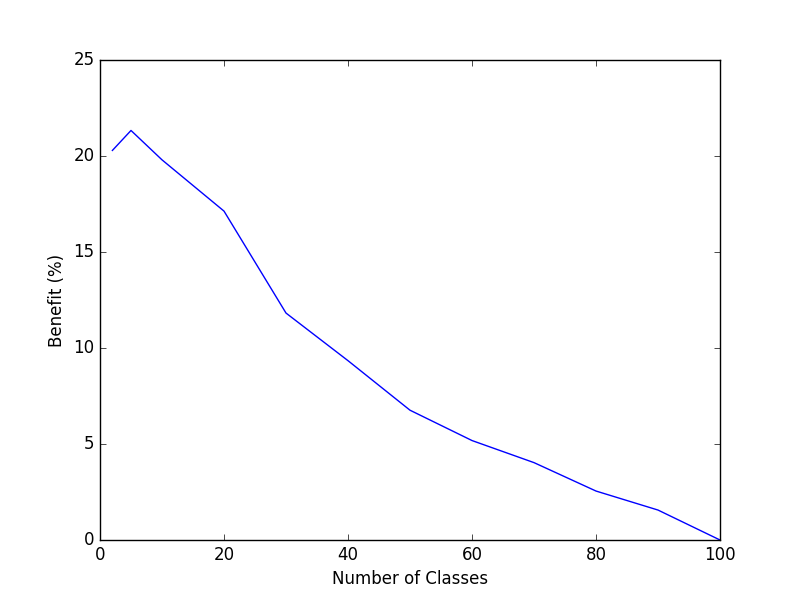
\includegraphics[scale=0.43]{figure_1.png}
\caption{Probability Layer Result}
\label{fig:ProbabilityLayer}
\end{figure}


\begin{table*}[!th]
    \centering
    \begin{tabular}{l|c|c|c}
        \hline
        \multicolumn{1}{c|}{Test Data} & Parameter  & Accuracy & Benefit \\
        Original CIFAR100 & 0 & 73.74\% &  \\
        \hline
        2 classes (0, 1) & 0 & 88.12\% &  \\
        2 classes (0, 1) & 1.0 & 98.51\% & +10.39\% \\
        \hline
        2 classes (3, 5) & 0 & 61.39\% &  \\
        2 classes (3, 5) & 1.0 & 99.01\% & +37.62\% \\
        \hline
        2 classes (0, 99) & 0 & 84.65\% & \\
        2 classes (0, 99) & 1.0 & 97.52\% & +12.87\% \\
        \hline
        5 classes $(0, ..., 4)$ & 0 & 66.33\% &  \\
        5 classes $(0, ..., 4)$ & 1.0 & 93.03\% & +26.70\% \\
        \hline
        5 classes $(5, ..., 9)$ & 0 & 81.06\% &  \\
        5 classes $(5, ..., 9)$ & 1.0 & 97.01\% & +15.95\% \\
        \hline
        10 classes $(0, ..., 9)$ & 0 & 75.35\% &  \\
        10 classes $(0, ..., 0)$ & 1.0 & 94.21\% & +18.86\% \\
        \hline
        10 classes $(10, ..., 19)$ & 0 & 67.16\% &  \\
        10 classes $(10, ..., 19)$ & 1.0 & 91.42\% & +24.26\% \\
        \hline
        10 classes $(20, ..., 29)$ & 0 & 75.84\% &  \\
        10 classes $(20, ..., 29)$ & 1.0 & 92.22\% & +16.38\% \\
        \hline
        
        
    \end{tabular}
    \vspace{1em}
    \caption{Test Probability Layer on Different Locality}
    \label{tab:ProbabilityLayer1}
\end{table*}


Experiments show the significant of \textit{probability layer} over \textit{naive mask}. Figure \ref{fig:NaiveMask} shows the comparison between probability layer and naive mask under different configurations. The red dash line represents the original accuracy without probability layer and naive mask, which is 74.57\%. When the number of domain classes is 10 and the distribution skew is 50\%, the accuracy with probability layer is 75.28\%, while the accuracy with naive mask is only 47.49\%. Thus probability layer has a positive effect even if the distribution skew is only 50\%, while the naive mask has a strong negative effect in this context. As we increase distribution skew gradually, the accuracy with probability layer and naive mask keeps increasing. Only after the distribution skew becomes larger than 77.67\%, naive mask starts to show positive effect on accuracy while probability layer keeps showing positive effect in all settings. As distribution skew approaches 100\%, the effect of naive mask catches probability layer up, since the true labels start to only exist in domain classes. In short, probability layer is a generalization of naive mask and shows benefit over original model and naive mask consistently.

\begin{figure}
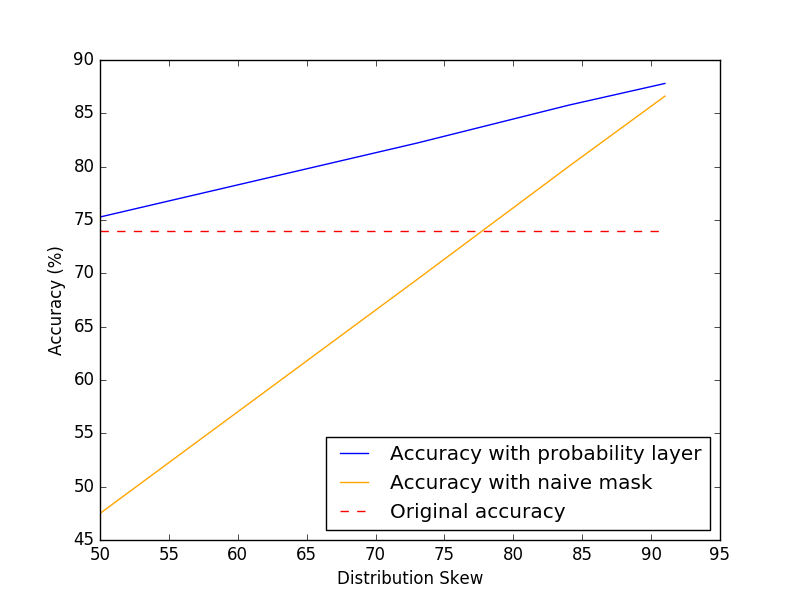
\includegraphics[scale=0.43]{figure_1-1.png}
\caption{Comparison Between Probability Layer and Naive Mask}
\label{fig:NaiveMask}
\end{figure}


\begin{figure}
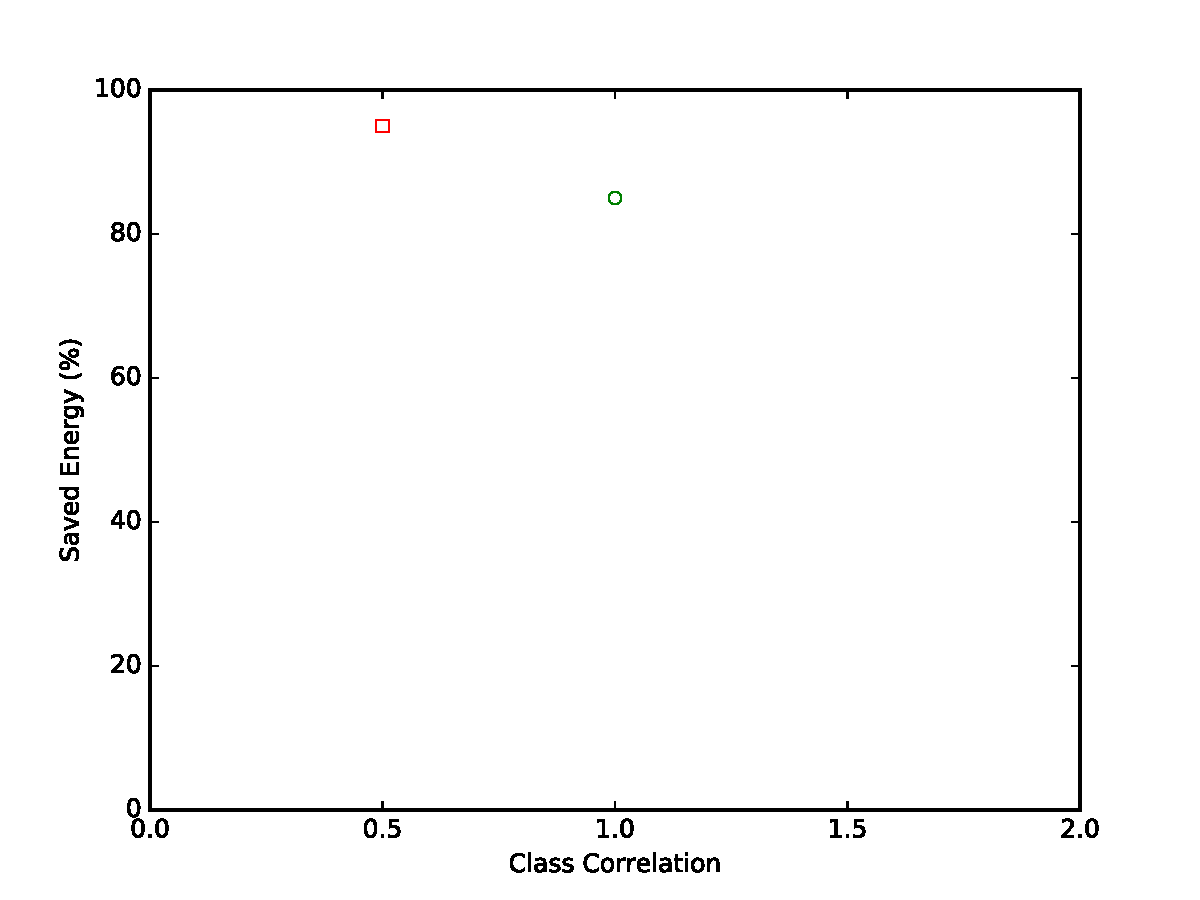
\includegraphics[scale=0.43]{savedEnergy.ps}
\caption{Saved Energy}
\label{fig:savedEnergy}
\end{figure}


\subsection{Energy efficiency}
Considering class correlation can save more energy than only considering number of classes. Fig \ref{fig:savedEnergy} shows the energy saved by class correlation. We generate a subset from CIFAR100 with 2 classes and different class correlation. The accuracy of VGG16 on CIFAR100 is 70.48\%. We simplify VGG16 and reduce layers until the testing accuracy on specialized dataset is lower than 70\%. Considering the innegligible impact of class correlation on testing accuracy, the experiments are done by different class correlation and, for each class correlation, the classes are selected randomly and the experiments are repeated for twenty times to get an average accuracy. When the class number is two and class correlation is $1$, we need a model with one convolutional layer and two fully connected layer to get the accuracy as $72.9\%$. Thus we only need to consume $85\%$ computation to get the same accuracy as the VGG16 with $19$ layers. If we decrease the class correlation to $0.5$, we only need a single fully connected layer to achieve 74.6\% accuracy. In this case, only $5\%$ computation of VGG16 is consumed. Thus, as we decrease class correlation from $1$ to $0.5$, the energy consumption is decreased by $66\%$


\section{Comparison with previous work}
\subsection{Distillation}
Distillation has been discussed extensively in machine learning area \cite{hinton2015distilling, ba2014deep, dauphin2013big, chen2017learning, lopez2015unifying, kim2015compression,bucilu2006model}. With distillation, we can use a smaller model to learn a complex model, get a better performance than the small model, and consume less energy than the complex model. Thus distillation naturally fits great with energy-efficiency on mobile device. However, neither the distillation people nor the mobile energy efficiency people considered combining these two techniques together. We are the first to introduce distillation into mobile energy efficiency. We solved obstacles in both side. First, existing distillation methods could only learn a large model when there are equal number of nodes in the softmax layer while our method could proceed no matter the difference between these two numbers. Second, existing papers could either only retrain last few layers \cite{li2015towards}, which lose the ability to change model architecture, or retrain the model from scratch \cite{han2016mcdnn, kang2017noscope, shen2017fast}, which lose the information contained in large model. Introducing distillation into runtime optimization can solve these problems perfectly.

\subsection{Specialization}
Use specialization to generate a series of models composing trade-off between accuracy and energy is an emerging method for solving energy efficiency problem on mobile devices \cite{han2016mcdnn, kang2017noscope, shen2017fast}. Generally the reduction in energy is achieved by reducing number of layers and the resulting decrease in accuracy is made up by reducing number of nodes in the softmax layer. Although existing papers introduced a new way to solve the energy efficiency problem, the implementation detail is very coarse-grained and there are lots of open questions to be answered. Instead of only considering number of classes in the runtime, our paper took class correlation into consideration and introduced semantic tree as a quantitative method describing similarity between classes. Based on the numeric metric, we brought up guided search to replace exhaustive search used in existing papers. The second contribution is to introduce distillation and varying input size into runtime optimization. Previously, the only method employed in this area is to reducing number of layers. We found that input size is also a simple but effective in specialization. Finally, \textit{probability layer} was proposed to act as cold-start, solved the time latency introduced by retraining, and gives more choice for the scheduling model.

\subsection{Model Compression}
Model compression is to compress CNN architecture through matrix factorization and matrix pruning. Matrix factorization \cite{jaderberg2014speeding, kim2015compression, romero2014fitnets, xue2014singular} means using the multiplication of two low rank matrices to replace a single high rank matrix. Matrix pruning \cite{chen2015compressing, han2015learning} is to transform a matrix into sparse matrix by pruning small digits to be zero. Both directions of model compression do not change the number of nodes in the softmax layer or the model architecture. Thus techniques in model compression is orthogonal to using runtime distribution and could provide further optimization after reducing number of classes. 


\subsection{Early Stop} 
Early stop \cite{teerapittayanon2016branchynet, panda2016conditional} is an architecture with branches and will stop calculating once a branch is enough confident that an image has been classified correctly. Early stop contains various architectures to achieve energy efficiency through reducing unnecessary computation. This is orthogonal to runtime specialization and could be included into the model bank.



\section{Conclusion and Future Work}
By using runtime class skew, including reduction in number of classes and similarity between a cluster of classes, we can increase accuracy without any change in model architecture. This phenonmenon gives us space to dramatically simplify our CNN models by changing input size, reducing number of nodes in softmax layer, reducing number of layers, and distillation.  Further, we can use probability layer to make use of this class skew without retraining if the energy budget is limited, or retrain the last few layers if energy constraint is loose. By recording the repeated pattern of classes, cold retrain the model is a feasible way to make use of runtime distribution without runtime retrain. Finnaly, the end-to-end runtime support framework, SMART, can reduce energy consumption by xx times while increase the accuracy by xx times. (EXPERIMENTS TO BE ADDED). In the future, we will provide a more detailed mapping from class cluster to suggested models.


% An example of a floating figure using the graphicx package.
% Note that \label must occur AFTER (or within) \caption.
% For figures, \caption should occur after the \includegraphics.
% Note that IEEEtran v1.7 and later has special internal code that
% is designed to preserve the operation of \label within \caption
% even when the captionsoff option is in effect. However, because
% of issues like this, it may be the safest practice to put all your
% \label just after \caption rather than within \caption{}.
%
% Reminder: the "draftcls" or "draftclsnofoot", not "draft", class
% option should be used if it is desired that the figures are to be
% displayed while in draft mode.
%
%\begin{figure}[!t]
%\centering
%\includegraphics[width=2.5in]{myfigure}
% where an .eps filename suffix will be assumed under latex,
% and a .pdf suffix will be assumed for pdflatex; or what has been declared
% via \DeclareGraphicsExtensions.
%\caption{Simulation results for the network.}
%\label{fig_sim}
%\end{figure}

% Note that the IEEE typically puts floats only at the top, even when this
% results in a large percentage of a column being occupied by floats.


% An example of a double column floating figure using two subfigures.
% (The subfig.sty package must be loaded for this to work.)
% The subfigure \label commands are set within each subfloat command,
% and the \label for the overall figure must come after \caption.
% \hfil is used as a separator to get equal spacing.
% Watch out that the combined width of all the subfigures on a
% line do not exceed the text width or a line break will occur.
%
%\begin{figure*}[!t]
%\centering
%\subfloat[Case I]{\includegraphics[width=2.5in]{box}%
%\label{fig_first_case}}
%\hfil
%\subfloat[Case II]{\includegraphics[width=2.5in]{box}%
%\label{fig_second_case}}
%\caption{Simulation results for the network.}
%\label{fig_sim}
%\end{figure*}
%
% Note that often IEEE papers with subfigures do not employ subfigure
% captions (using the optional argument to \subfloat[]), but instead will
% reference/describe all of them (a), (b), etc., within the main caption.
% Be aware that for subfig.sty to generate the (a), (b), etc., subfigure
% labels, the optional argument to \subfloat must be present. If a
% subcaption is not desired, just leave its contents blank,
% e.g., \subfloat[].


% An example of a floating table. Note that, for IEEE style tables, the
% \caption command should come BEFORE the table and, given that table
% captions serve much like titles, are usually capitalized except for words
% such as a, an, and, as, at, but, by, for, in, nor, of, on, or, the, to
% and up, which are usually not capitalized unless they are the first or
% last word of the caption. Table text will default to \footnotesize as
% the IEEE normally uses this smaller font for tables.
% The \label must come after \caption as always.
%
%\begin{table}[!t]
%% increase table row spacing, adjust to taste
%\renewcommand{\arraystretch}{1.3}
% if using array.sty, it might be a good idea to tweak the value of
% \extrarowheight as needed to properly center the text within the cells
%\caption{An Example of a Table}
%\label{table_example}
%\centering
%% Some packages, such as MDW tools, offer better commands for making tables
%% than the plain LaTeX2e tabular which is used here.
%\begin{tabular}{|c||c|}
%\hline
%One & Two\\
%\hline
%Three & Four\\
%\hline
%\end{tabular}
%\end{table}


% Note that the IEEE does not put floats in the very first column
% - or typically anywhere on the first page for that matter. Also,
% in-text middle ("here") positioning is typically not used, but it
% is allowed and encouraged for Computer Society conferences (but
% not Computer Society journals). Most IEEE journals/conferences use
% top floats exclusively.
% Note that, LaTeX2e, unlike IEEE journals/conferences, places
% footnotes above bottom floats. This can be corrected via the
% \fnbelowfloat command of the stfloats package.




%\section{Conclusion}
%The conclusion goes here.




% conference papers do not normally have an appendix





% trigger a \newpage just before the given reference
% number - used to balance the columns on the last page
% adjust value as needed - may need to be readjusted if
% the document is modified later
%\IEEEtriggeratref{8}
% The "triggered" command can be changed if desired:
%\IEEEtriggercmd{\enlargethispage{-5in}}

% references section

% can use a bibliography generated by BibTeX as a .bbl file
% BibTeX documentation can be easily obtained at:
% http://mirror.ctan.org/biblio/bibtex/contrib/doc/
% The IEEEtran BibTeX style support page is at:
% http://www.michaelshell.org/tex/ieeetran/bibtex/
%\bibliographystyle{IEEEtran}
% argument is your BibTeX string definitions and bibliography database(s)
%\bibliography{IEEEabrv,../bib/paper}
%
% <OR> manually copy in the resultant .bbl file
% set second argument of \begin to the number of references
% (used to reserve space for the reference number labels box)
%\begin{thebibliography}{1}
%
%\bibitem{IEEEhowto:kopka}
%H.~Kopka and P.~W. Daly, \emph{A Guide to \LaTeX}, 3rd~ed.\hskip 1em plus
%  0.5em minus 0.4em\relax Harlow, England: Addison-Wesley, 1999.
%
%\end{thebibliography}


\bibliographystyle{IEEEtran.bst}
\bibliography{main}


\end{spacing}

% that's all folks
\end{document}
\grid
